\documentclass{article}

\usepackage{fancyhdr}
\usepackage{wrapfig}
\usepackage{extramarks}
\usepackage{multicol}
\usepackage{amsmath}
\usepackage{amsthm}
\usepackage{amsfonts}
\usepackage{tikz}
\usepackage[plain]{algorithm}
\usepackage{algpseudocode}
\usepackage{enumerate}
\usepackage[shortlabels]{enumitem}                                          
                    \setlist[enumerate, 1]{1\textsuperscript{o}}



\usepackage{listings}
\usepackage{xcolor}
\lstset { %
    language=C++,
    backgroundcolor=\color{black!5}, % set backgroundcolor
    basicstyle=\footnotesize,% basic font setting
}

%\usetikzlibrary{automata,positioning}
\usetikzlibrary{positioning,shapes,shadows,arrows,automata}

%
% Basic Document Settings
%

\topmargin=-0.45in
\evensidemargin=0in
\oddsidemargin=0in
\textwidth=6.5in
\textheight=9.0in
\headsep=0.25in

\linespread{1.1}

\pagestyle{fancy}
\lhead{\hmwkAuthorName}
\chead{\hmwkClass\ (\hmwkClassInstructor\ \hmwkClassTime): \hmwkTitle}
\rhead{\firstxmark}
\lfoot{\lastxmark}
\cfoot{\thepage}

\renewcommand\headrulewidth{0.4pt}
\renewcommand\footrulewidth{0.4pt}

\setlength\parindent{0pt}

%
% Create Problem Sections
%

\newcommand{\enterProblemHeader}[1]{
    \nobreak\extramarks{}{Problem \arabic{#1} continued on next page\ldots}\nobreak{}
    \nobreak\extramarks{Problem \arabic{#1} (continued)}{Problem \arabic{#1} continued on next page\ldots}\nobreak{}
}

\newcommand{\exitProblemHeader}[1]{
    \nobreak\extramarks{Problem \arabic{#1} (continued)}{Problem \arabic{#1} continued on next page\ldots}\nobreak{}
    \stepcounter{#1}
    \nobreak\extramarks{Problem \arabic{#1}}{}\nobreak{}
}

\setcounter{secnumdepth}{0}
\newcounter{partCounter}
\newcounter{homeworkProblemCounter}
\setcounter{homeworkProblemCounter}{1}
\nobreak\extramarks{Problem \arabic{homeworkProblemCounter}}{}\nobreak{}

%
% Homework Problem Environment
%
% This environment takes an optional argument. When given, it will adjust the
% problem counter. This is useful for when the problems given for your
% assignment aren't sequential. See the last 3 problems of this template for an
% example.
%
\newenvironment{homeworkProblem}[1][-1]{
    \ifnum#1>0
        \setcounter{homeworkProblemCounter}{#1}
    \fi
    \section{Problem \arabic{homeworkProblemCounter}}
    \setcounter{partCounter}{1}
    \enterProblemHeader{homeworkProblemCounter}
}{
    \exitProblemHeader{homeworkProblemCounter}
}

%
% Homework Details
%   - Title
%   - Due date
%   - Class
%   - Section/Time
%   - Instructor
%   - Author
%

\newcommand{\hmwkTitle}{Homework\ \#1}
\newcommand{\hmwkDueDate}{January 20 2015}
\newcommand{\hmwkClass}{CS581 Theory of Computation}
\newcommand{\hmwkClassTime}{Winter 2016}
\newcommand{\hmwkClassInstructor}{Harry H. Porter}
\newcommand{\hmwkAuthorName}{Konstantin Macarenco}

%
% Title Page
%

\title{
    \vspace{2in}
    \textmd{\textbf{\hmwkClass:\ \hmwkTitle}}\\
    \normalsize\vspace{0.1in}\small{Due\ on\ \hmwkDueDate\ at 2:00pm}\\
    \vspace{0.1in}\large{\textit{\hmwkClassInstructor\ \hmwkClassTime}}
    \vspace{3in}
}

\author{\textbf{\hmwkAuthorName}}
\date{}

\renewcommand{\part}[1]{\textbf{\large Part \Alph{partCounter}}\stepcounter{partCounter}\\}

%
% Various Helper Commands
%

% Useful for algorithms
\newcommand{\alg}[1]{\textsc{\bfseries \footnotesize #1}}

% For derivatives
\newcommand{\deriv}[1]{\frac{\mathrm{d}}{\mathrm{d}x} (#1)}

% For partial derivatives
\newcommand{\pderiv}[2]{\frac{\partial}{\partial #1} (#2)}

% Integral dx
\newcommand{\dx}{\mathrm{d}x}

% Alias for the Solution section header
\newcommand{\solution}{\textbf{\large Solution}}

% Probability commands: Expectation, Variance, Covariance, Bias
\newcommand{\E}{\mathrm{E}}
\newcommand{\Var}{\mathrm{Var}}
\newcommand{\Cov}{\mathrm{Cov}}
\newcommand{\Bias}{\mathrm{Bias}}

\begin{document}

\maketitle

\pagebreak

\begin{homeworkProblem}

\noindent

\begin{center}
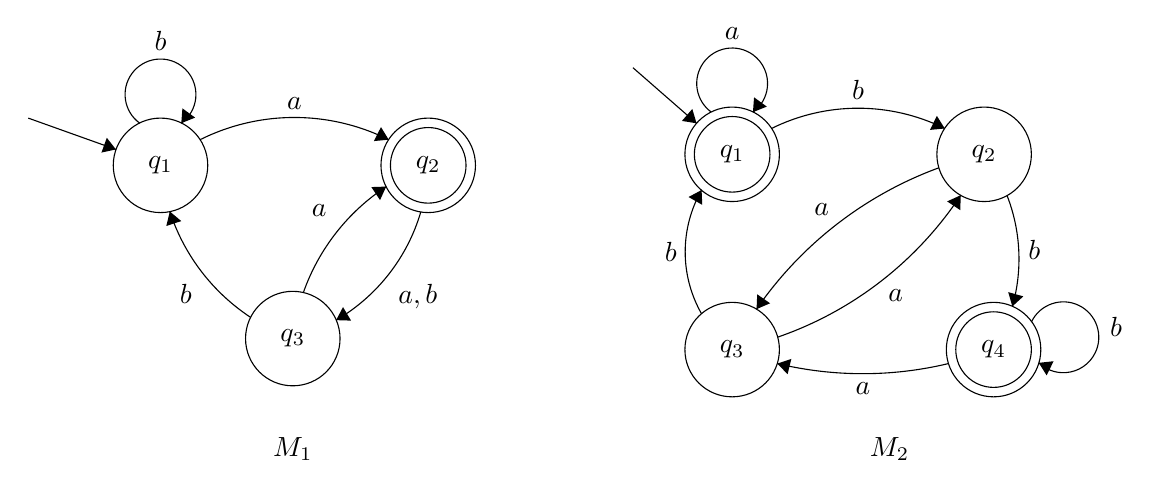
\begin{tikzpicture}[scale=0.2]
\tikzstyle{every node}+=[inner sep=0pt]
\draw [black] (9.8,-10.1) circle (3);
\draw (9.8,-10.1) node {$q_1$};
\draw [black] (26.8,-10.1) circle (3);
\draw (26.8,-10.1) node {$q_2$};
\draw [black] (26.8,-10.1) circle (2.4);
\draw [black] (18.2,-21.1) circle (3);
\draw (18.2,-21.1) node {$q_3$};
\draw (18.2,-28.1) node {$M_1$};
\draw [black] (46.1,-9.4) circle (3);
\draw (46.1,-9.4) node {$q_1$};
\draw [black] (46.1,-9.4) circle (2.4);
\draw [black] (62.1,-9.4) circle (3);
\draw (62.1,-9.4) node {$q_2$};
\draw [black] (46.1,-21.8) circle (3);
\draw (46.1,-21.8) node {$q_3$};
\draw (56.1,-28.1) node {$M_2$};
\draw [black] (62.7,-21.8) circle (3);
\draw (62.7,-21.8) node {$q_4$};
\draw [black] (62.7,-21.8) circle (2.4);
\draw [black] (8.477,-7.42) arc (234:-54:2.25);
\draw (9.8,-2.85) node [above] {$b$};
\fill [black] (11.12,-7.42) -- (12,-7.07) -- (11.19,-6.48);
\draw [black] (12.312,-8.472) arc (116.53845:63.46155:13.402);
\fill [black] (24.29,-8.47) -- (23.8,-7.67) -- (23.35,-8.56);
\draw (18.3,-6.56) node [above] {$a$};
\draw [black] (26.329,-13.055) arc (-16.32928:-59.70861:11.807);
\fill [black] (20.95,-19.93) -- (21.9,-19.96) -- (21.39,-19.1);
\draw (24.87,-18.42) node [right] {$a,b$};
\draw [black] (18.87,-18.182) arc (160.62375:123.33837:13.357);
\fill [black] (24.13,-11.45) -- (23.19,-11.48) -- (23.74,-12.31);
\draw (20.38,-12.97) node [left] {$a$};
\draw [black] (15.525,-19.756) arc (-123.37352:-161.89315:12.821);
\fill [black] (10.39,-13.03) -- (10.17,-13.95) -- (11.12,-13.64);
\draw (11.82,-18.24) node [left] {$b$};
\draw [black] (1.4,-7.1) -- (6.97,-9.09);
\fill [black] (6.97,-9.09) -- (6.39,-8.35) -- (6.05,-9.29);
\draw [black] (39.8,-3.9) -- (43.84,-7.43);
\fill [black] (43.84,-7.43) -- (43.57,-6.52) -- (42.91,-7.28);
\draw [black] (44.777,-6.72) arc (234:-54:2.25);
\draw (46.1,-2.15) node [above] {$a$};
\fill [black] (47.42,-6.72) -- (48.3,-6.37) -- (47.49,-5.78);
\draw [black] (48.602,-7.758) arc (116.33712:63.66288:12.392);
\fill [black] (59.6,-7.76) -- (59.1,-6.96) -- (58.66,-7.85);
\draw (54.1,-5.97) node [above] {$b$};
\draw [black] (63.554,-12.014) arc (21.33103:-15.7906:11.079);
\fill [black] (63.89,-19.06) -- (64.59,-18.42) -- (63.63,-18.15);
\draw (64.87,-15.49) node [right] {$b$};
\draw [black] (65.109,-20.032) arc (154.00798:-133.99202:2.25);
\draw (70.07,-20.37) node [right] {$b$};
\fill [black] (65.57,-22.64) -- (66.07,-23.44) -- (66.51,-22.54);
\draw [black] (59.836,-22.687) arc (-76.49247:-103.50753:23.274);
\fill [black] (48.96,-22.69) -- (49.62,-23.36) -- (49.86,-22.39);
\draw (54.4,-23.83) node [below] {$a$};
\draw [black] (60.612,-12.003) arc (-33.50518:-70.94346:22.905);
\fill [black] (60.61,-12) -- (59.75,-12.39) -- (60.59,-12.95);
\draw (56.49,-17.96) node [below] {$a$};
\draw [black] (47.646,-19.231) arc (145.41007:110.14129:24.182);
\fill [black] (47.65,-19.23) -- (48.51,-18.86) -- (47.69,-18.29);
\draw (51.79,-13.35) node [above] {$a$};
\draw [black] (44.161,-19.534) arc (-150.27637:-209.72363:7.935);
\fill [black] (44.16,-11.67) -- (43.33,-12.11) -- (44.2,-12.61);
\draw (42.62,-15.6) node [left] {$b$};
\end{tikzpicture}
\end{center}

\hspace{1cm}
\begin{enumerate}[a., leftmargin = 0.5cm, nosep]
\itemsep0em
\item Start State: $M_1$ - $q_1$, $M_2$ - $q_1$
\item Set of accept states $M_1$ - $F=\{q_2\}$, $M_2$ - $F=\{q_1,q_4\}$, 
\item $M_1$ = $\{q_1,q_2,q_3,q_1,q_1\}$, $M_2$ $=\{q_1,q_1,q_1,q_2,q_4\}$
\item $M_1$ No, $M_2$ Yes
\item $M_1$ No, $M_2$ Yes
\end{enumerate}
\end{homeworkProblem}

\begin{homeworkProblem}
$M_1$
\begin{enumerate}[1., leftmargin = 0.5cm]
\itemsep0em
\item $Q = \{q_1,q_2,q_3\}$
\item $\sum = \{a,b\}$
\item $\delta$ described as
\begin{table}[h!]
\centering
\caption{$M_1$ Transition function}
\label{my-label}
\begin{tabular}{l|ll}
      & a     &    b  \\ \hline
$q_1$ & $q_2$ & $q_1$ \\
$q_2$ & $q_3$ & $q_3$ \\
$q_3$ & $q_2$ & $q_1$
\end{tabular}
\end{table}
\item Start state $q_1 \in Q$
\item $F = \{q_3\} \subseteq Q$ Start state $q_1 \in Q$
\end{enumerate}
\pagebreak
$M_2$
\begin{enumerate}[1., leftmargin = 0.5cm]
\itemsep0em
\item $Q = \{q_1,q_2,q_3,q_4\}$
\item $\sum = \{a,b\}$
\item $\delta$ described as
\begin{table}[h!]
\centering
\caption{$M_2$ Transition function}
\label{my-label}
\begin{tabular}{l|ll}
      & a     &    b  \\ \hline
$q_1$ & $q_1$ & $q_2$ \\
$q_2$ & $q_3$ & $q_4$ \\
$q_3$ & $q_2$ & $q_1$ \\
$q_4$ & $q_3$ & $q_4$
\end{tabular}
\end{table}
\item Start state $q_1 \in Q$
\item $F = \{q_1,q_4\} \subseteq Q$ Start state $q_1 \in Q$
\end{enumerate}

\end{homeworkProblem}

\begin{homeworkProblem}

\begin{center}
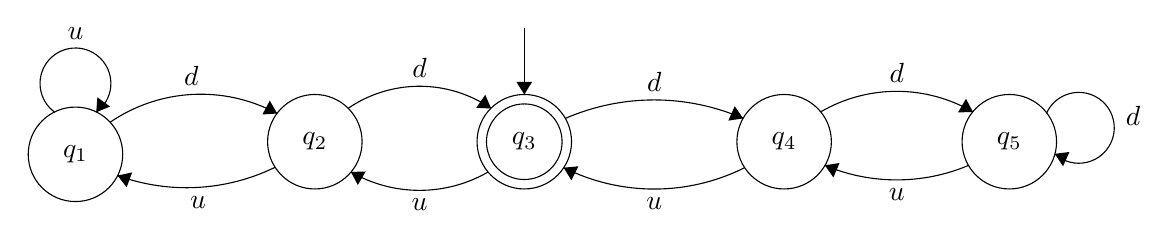
\begin{tikzpicture}[scale=0.2]
\tikzstyle{every node}+=[inner sep=0pt]
\draw [black] (8.3,-10.1) circle (3);
\draw (8.3,-10.1) node {$q_1$};
\draw [black] (23.5,-9.3) circle (3);
\draw (23.5,-9.3) node {$q_2$};
\draw [black] (36.8,-9.3) circle (3);
\draw (36.8,-9.3) node {$q_3$};
\draw [black] (36.8,-9.3) circle (2.4);
\draw [black] (53.3,-9.3) circle (3);
\draw (53.3,-9.3) node {$q_4$};
\draw [black] (67.6,-9.3) circle (3);
\draw (67.6,-9.3) node {$q_5$};
\draw [black] (36.8,-2.1) -- (36.8,-6.3);
\fill [black] (36.8,-6.3) -- (37.3,-5.5) -- (36.3,-5.5);
\draw [black] (6.977,-7.42) arc (234:-54:2.25);
\draw (8.3,-2.85) node [above] {$u$};
\fill [black] (9.62,-7.42) -- (10.5,-7.07) -- (9.69,-6.48);
\draw [black] (10.492,-8.068) arc (124.40866:61.61691:10.202);
\fill [black] (21.11,-7.51) -- (20.64,-6.69) -- (20.17,-7.57);
\draw (15.66,-5.75) node [above] {$d$};
\draw [black] (20.983,-10.92) arc (-63.94561:-110.02881:12.805);
\fill [black] (10.97,-11.45) -- (11.55,-12.19) -- (11.9,-11.25);
\draw (16.09,-12.75) node [below] {$u$};
\draw [black] (25.604,-7.186) arc (124.43892:55.56108:8.038);
\fill [black] (34.7,-7.19) -- (34.32,-6.32) -- (33.75,-7.15);
\draw (30.15,-5.28) node [above] {$d$};
\draw [black] (34.512,-11.217) arc (-59.92561:-120.07439:8.703);
\fill [black] (25.79,-11.22) -- (26.23,-12.05) -- (26.73,-11.19);
\draw (30.15,-12.89) node [below] {$u$};
\draw [black] (39.404,-7.821) arc (113.51604:66.48396:14.15);
\fill [black] (50.7,-7.82) -- (50.16,-7.04) -- (49.76,-7.96);
\draw (45.05,-6.15) node [above] {$d$};
\draw [black] (50.8,-10.945) arc (-63.35828:-116.64172:12.822);
\fill [black] (39.3,-10.95) -- (39.79,-11.75) -- (40.24,-10.86);
\draw (45.05,-12.81) node [below] {$u$};
\draw [black] (55.613,-7.409) arc (120.29559:59.70441:9.588);
\fill [black] (65.29,-7.41) -- (64.85,-6.57) -- (64.34,-7.44);
\draw (60.45,-5.6) node [above] {$d$};
\draw [black] (65.013,-10.803) arc (-67.15252:-112.84748:11.752);
\fill [black] (55.89,-10.8) -- (56.43,-11.57) -- (56.82,-10.65);
\draw (60.45,-12.23) node [below] {$u$};
\draw [black] (69.968,-7.478) arc (155.30993:-132.69007:2.25);
\draw (74.96,-7.66) node [right] {$d$};
\fill [black] (70.49,-10.07) -- (71.01,-10.86) -- (71.42,-9.95);
\end{tikzpicture}
\end{center}
\end{homeworkProblem}


\begin{homeworkProblem}
\textbf{a}
\begin{center}
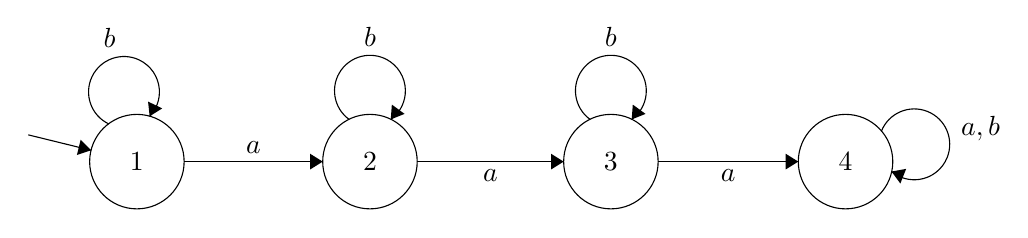
\begin{tikzpicture}[scale=0.2]
\tikzstyle{every node}+=[inner sep=0pt]
\draw [black] (9.1,-9.3) circle (3);
\draw (9.1,-9.3) node {$1$};
\draw [black] (23.9,-9.3) circle (3);
\draw (23.9,-9.3) node {$2$};
\draw [black] (39.2,-9.3) circle (3);
\draw (39.2,-9.3) node {$3$};
\draw [black] (54.1,-9.3) circle (3);
\draw (54.1,-9.3) node {$4$};
\draw [black] (12.1,-9.3) -- (20.9,-9.3);
\fill [black] (20.9,-9.3) -- (20.1,-8.8) -- (20.1,-9.8);
\draw (16.5,-8.8) node [above] {$a$};
\draw [black] (26.9,-9.3) -- (36.2,-9.3);
\fill [black] (36.2,-9.3) -- (35.4,-8.8) -- (35.4,-9.8);
\draw (31.55,-9.8) node [below] {$a$};
\draw [black] (42.2,-9.3) -- (51.1,-9.3);
\fill [black] (51.1,-9.3) -- (50.3,-8.8) -- (50.3,-9.8);
\draw (46.65,-9.8) node [below] {$a$};
\draw [black] (56.377,-7.364) arc (158.10808:-129.89192:2.25);
\draw (61.41,-7.19) node [right] {$a,b$};
\fill [black] (57.02,-9.93) -- (57.58,-10.69) -- (57.95,-9.76);
\draw [black] (37.877,-6.62) arc (234:-54:2.25);
\draw (39.2,-2.05) node [above] {$b$};
\fill [black] (40.52,-6.62) -- (41.4,-6.27) -- (40.59,-5.68);
\draw [black] (22.577,-6.62) arc (234:-54:2.25);
\draw (23.9,-2.05) node [above] {$b$};
\fill [black] (25.22,-6.62) -- (26.1,-6.27) -- (25.29,-5.68);
\draw [black] (7.312,-6.906) arc (244.49148:-43.50852:2.25);
\draw (7.36,-2.07) node [above] {$b$};
\fill [black] (9.91,-6.42) -- (10.71,-5.92) -- (9.81,-5.49);
\draw [black] (2.2,-7.6) -- (6.19,-8.58);
\fill [black] (6.19,-8.58) -- (5.53,-7.91) -- (5.29,-8.88);
\end{tikzpicture}
\end{center}

\begin{center}
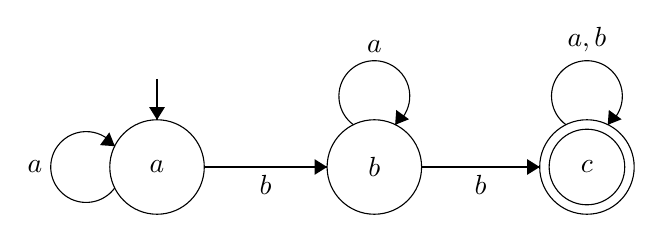
\begin{tikzpicture}[scale=0.2]
\tikzstyle{every node}+=[inner sep=0pt]
\draw [black] (11.8,-10.1) circle (3);
\draw (11.8,-10.1) node {$a$};
\draw [black] (25.6,-10.1) circle (3);
\draw (25.6,-10.1) node {$b$};
\draw [black] (39.1,-10.1) circle (3);
\draw (39.1,-10.1) node {$c$};
\draw [black] (39.1,-10.1) circle (2.4);
\draw [black] (11.8,-4.5) -- (11.8,-7.1);
\fill [black] (11.8,-7.1) -- (12.3,-6.3) -- (11.3,-6.3);
\draw [black] (14.8,-10.1) -- (22.6,-10.1);
\fill [black] (22.6,-10.1) -- (21.8,-9.6) -- (21.8,-10.6);
\draw (18.7,-10.6) node [below] {$b$};
\draw [black] (28.6,-10.1) -- (36.1,-10.1);
\fill [black] (36.1,-10.1) -- (35.3,-9.6) -- (35.3,-10.6);
\draw (32.35,-10.6) node [below] {$b$};
\draw [black] (37.777,-7.42) arc (234:-54:2.25);
\draw (39.1,-2.85) node [above] {$a,b$};
\fill [black] (40.42,-7.42) -- (41.3,-7.07) -- (40.49,-6.48);
\draw [black] (9.12,-11.423) arc (324:36:2.25);
\draw (4.55,-10.1) node [left] {$a$};
\fill [black] (9.12,-8.78) -- (8.77,-7.9) -- (8.18,-8.71);
\draw [black] (24.277,-7.42) arc (234:-54:2.25);
\draw (25.6,-2.85) node [above] {$a$};
\fill [black] (26.92,-7.42) -- (27.8,-7.07) -- (26.99,-6.48);
\end{tikzpicture}
\end{center}

\begin{center}
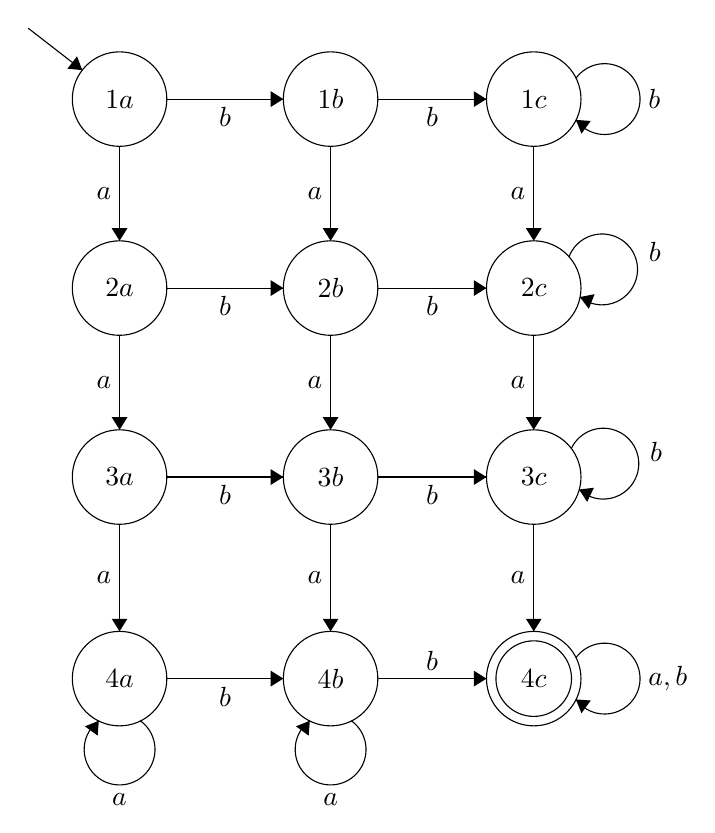
\begin{tikzpicture}[scale=0.2]
\tikzstyle{every node}+=[inner sep=0pt]
\draw [black] (7.4,-5.7) circle (3);
\draw (7.4,-5.7) node {$1a$};
\draw [black] (20.8,-5.7) circle (3);
\draw (20.8,-5.7) node {$1b$};
\draw [black] (33.7,-5.7) circle (3);
\draw (33.7,-5.7) node {$1c$};
\draw [black] (7.4,-17.7) circle (3);
\draw (7.4,-17.7) node {$2a$};
\draw [black] (20.8,-17.7) circle (3);
\draw (20.8,-17.7) node {$2b$};
\draw [black] (33.7,-17.7) circle (3);
\draw (33.7,-17.7) node {$2c$};
\draw [black] (7.4,-29.7) circle (3);
\draw (7.4,-29.7) node {$3a$};
\draw [black] (20.8,-29.7) circle (3);
\draw (20.8,-29.7) node {$3b$};
\draw [black] (33.7,-29.7) circle (3);
\draw (33.7,-29.7) node {$3c$};
\draw [black] (20.8,-42.5) circle (3);
\draw (20.8,-42.5) node {$4b$};
\draw [black] (7.4,-42.5) circle (3);
\draw (7.4,-42.5) node {$4a$};
\draw [black] (33.7,-42.5) circle (3);
\draw (33.7,-42.5) node {$4c$};
\draw [black] (33.7,-42.5) circle (2.4);
\draw [black] (1.6,-1.2) -- (5.03,-3.86);
\fill [black] (5.03,-3.86) -- (4.7,-2.98) -- (4.09,-3.77);
\draw [black] (10.4,-5.7) -- (17.8,-5.7);
\fill [black] (17.8,-5.7) -- (17,-5.2) -- (17,-6.2);
\draw (14.1,-6.2) node [below] {$b$};
\draw [black] (23.8,-5.7) -- (30.7,-5.7);
\fill [black] (30.7,-5.7) -- (29.9,-5.2) -- (29.9,-6.2);
\draw (27.25,-6.2) node [below] {$b$};
\draw [black] (7.4,-8.7) -- (7.4,-14.7);
\fill [black] (7.4,-14.7) -- (7.9,-13.9) -- (6.9,-13.9);
\draw (6.9,-11.7) node [left] {$a$};
\draw [black] (10.4,-17.7) -- (17.8,-17.7);
\fill [black] (17.8,-17.7) -- (17,-17.2) -- (17,-18.2);
\draw (14.1,-18.2) node [below] {$b$};
\draw [black] (20.8,-8.7) -- (20.8,-14.7);
\fill [black] (20.8,-14.7) -- (21.3,-13.9) -- (20.3,-13.9);
\draw (20.3,-11.7) node [left] {$a$};
\draw [black] (23.8,-17.7) -- (30.7,-17.7);
\fill [black] (30.7,-17.7) -- (29.9,-17.2) -- (29.9,-18.2);
\draw (27.25,-18.2) node [below] {$b$};
\draw [black] (33.7,-8.7) -- (33.7,-14.7);
\fill [black] (33.7,-14.7) -- (34.2,-13.9) -- (33.2,-13.9);
\draw (33.2,-11.7) node [left] {$a$};
\draw [black] (7.4,-20.7) -- (7.4,-26.7);
\fill [black] (7.4,-26.7) -- (7.9,-25.9) -- (6.9,-25.9);
\draw (6.9,-23.7) node [left] {$a$};
\draw [black] (20.8,-20.7) -- (20.8,-26.7);
\fill [black] (20.8,-26.7) -- (21.3,-25.9) -- (20.3,-25.9);
\draw (20.3,-23.7) node [left] {$a$};
\draw [black] (33.7,-20.7) -- (33.7,-26.7);
\fill [black] (33.7,-26.7) -- (34.2,-25.9) -- (33.2,-25.9);
\draw (33.2,-23.7) node [left] {$a$};
\draw [black] (10.4,-29.7) -- (17.8,-29.7);
\fill [black] (17.8,-29.7) -- (17,-29.2) -- (17,-30.2);
\draw (14.1,-30.2) node [below] {$b$};
\draw [black] (23.8,-29.7) -- (30.7,-29.7);
\fill [black] (30.7,-29.7) -- (29.9,-29.2) -- (29.9,-30.2);
\draw (27.25,-30.2) node [below] {$b$};
\draw [black] (20.8,-32.7) -- (20.8,-39.5);
\fill [black] (20.8,-39.5) -- (21.3,-38.7) -- (20.3,-38.7);
\draw (20.3,-36.1) node [left] {$a$};
\draw [black] (36.082,-27.895) arc (154.88553:-133.11447:2.25);
\draw (41.06,-28.13) node [right] {$b$};
\fill [black] (36.58,-30.49) -- (37.09,-31.28) -- (37.52,-30.38);
\draw [black] (22.123,-45.18) arc (54:-234:2.25);
\draw (20.8,-49.75) node [below] {$a$};
\fill [black] (19.48,-45.18) -- (18.6,-45.53) -- (19.41,-46.12);
\draw [black] (36.38,-4.377) arc (144:-144:2.25);
\draw (40.95,-5.7) node [right] {$b$};
\fill [black] (36.38,-7.02) -- (36.73,-7.9) -- (37.32,-7.09);
\draw [black] (35.937,-15.719) arc (159.25512:-128.74488:2.25);
\draw (40.98,-15.4) node [right] {$b$};
\fill [black] (36.63,-18.27) -- (37.2,-19.02) -- (37.56,-18.09);
\draw [black] (7.4,-32.7) -- (7.4,-39.5);
\fill [black] (7.4,-39.5) -- (7.9,-38.7) -- (6.9,-38.7);
\draw (6.9,-36.1) node [left] {$a$};
\draw [black] (10.4,-42.5) -- (17.8,-42.5);
\fill [black] (17.8,-42.5) -- (17,-42) -- (17,-43);
\draw (14.1,-43) node [below] {$b$};
\draw [black] (23.8,-42.5) -- (30.7,-42.5);
\fill [black] (30.7,-42.5) -- (29.9,-42) -- (29.9,-43);
\draw (27.25,-42) node [above] {$b$};
\draw [black] (33.7,-32.7) -- (33.7,-39.5);
\fill [black] (33.7,-39.5) -- (34.2,-38.7) -- (33.2,-38.7);
\draw (33.2,-36.1) node [left] {$a$};
\draw [black] (36.38,-41.177) arc (144:-144:2.25);
\draw (40.95,-42.5) node [right] {$a,b$};
\fill [black] (36.38,-43.82) -- (36.73,-44.7) -- (37.32,-43.89);
\draw [black] (8.723,-45.18) arc (54:-234:2.25);
\draw (7.4,-49.75) node [below] {$a$};
\fill [black] (6.08,-45.18) -- (5.2,-45.53) -- (6.01,-46.12);
\end{tikzpicture}
\end{center}



\textbf{b.}
\begin{center}
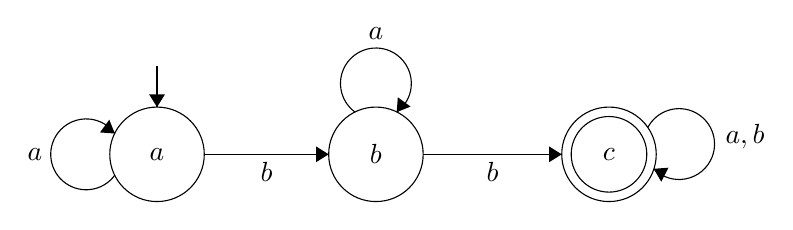
\begin{tikzpicture}[scale=0.2]
\tikzstyle{every node}+=[inner sep=0pt]
\draw [black] (10.5,-9.1) circle (3);
\draw (10.5,-9.1) node {$a$};
\draw [black] (24.4,-9.1) circle (3);
\draw (24.4,-9.1) node {$b$};
\draw [black] (39.2,-9.1) circle (3);
\draw (39.2,-9.1) node {$c$};
\draw [black] (39.2,-9.1) circle (2.4);
\draw [black] (10.5,-3.5) -- (10.5,-6.1);
\fill [black] (10.5,-6.1) -- (11,-5.3) -- (10,-5.3);
\draw [black] (13.5,-9.1) -- (21.4,-9.1);
\fill [black] (21.4,-9.1) -- (20.6,-8.6) -- (20.6,-9.6);
\draw (17.45,-9.6) node [below] {$b$};
\draw [black] (27.4,-9.1) -- (36.2,-9.1);
\fill [black] (36.2,-9.1) -- (35.4,-8.6) -- (35.4,-9.6);
\draw (31.8,-9.6) node [below] {$b$};
\draw [black] (41.66,-7.404) arc (152.31408:-135.68592:2.25);
\draw (46.57,-7.95) node [right] {$a,b$};
\fill [black] (42.04,-10.02) -- (42.52,-10.84) -- (42.98,-9.95);
\draw [black] (7.82,-10.423) arc (324:36:2.25);
\draw (3.25,-9.1) node [left] {$a$};
\fill [black] (7.82,-7.78) -- (7.47,-6.9) -- (6.88,-7.71);
\draw [black] (23.077,-6.42) arc (234:-54:2.25);
\draw (24.4,-1.85) node [above] {$a$};
\fill [black] (25.72,-6.42) -- (26.6,-6.07) -- (25.79,-5.48);
\end{tikzpicture}
\end{center}

\begin{center}
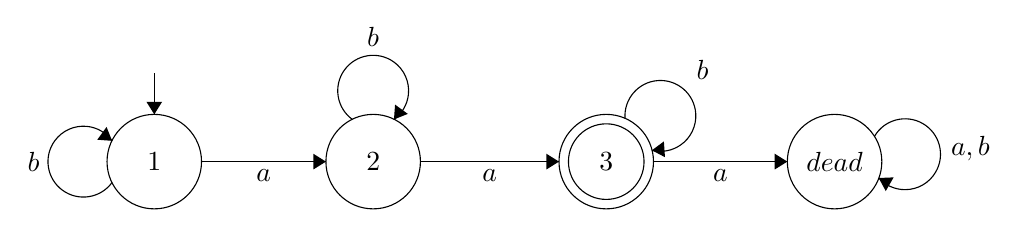
\begin{tikzpicture}[scale=0.2]
\tikzstyle{every node}+=[inner sep=0pt]
\draw [black] (10.5,-9.1) circle (3);
\draw (10.5,-9.1) node {$1$};
\draw [black] (24.4,-9.1) circle (3);
\draw (24.4,-9.1) node {$2$};
\draw [black] (39.2,-9.1) circle (3);
\draw (39.2,-9.1) node {$3$};
\draw [black] (39.2,-9.1) circle (2.4);
\draw [black] (53.7,-9.1) circle (3);
\draw (53.7,-9.1) node {$dead$};
\draw [black] (10.5,-3.5) -- (10.5,-6.1);
\fill [black] (10.5,-6.1) -- (11,-5.3) -- (10,-5.3);
\draw [black] (13.5,-9.1) -- (21.4,-9.1);
\fill [black] (21.4,-9.1) -- (20.6,-8.6) -- (20.6,-9.6);
\draw (17.45,-9.6) node [below] {$a$};
\draw [black] (27.4,-9.1) -- (36.2,-9.1);
\fill [black] (36.2,-9.1) -- (35.4,-8.6) -- (35.4,-9.6);
\draw (31.8,-9.6) node [below] {$a$};
\draw [black] (40.394,-6.361) arc (184.1777:-103.8223:2.25);
\draw (44.91,-3.3) node [right] {$b$};
\fill [black] (42.1,-8.38) -- (42.93,-8.82) -- (42.86,-7.82);
\draw [black] (7.82,-10.423) arc (324:36:2.25);
\draw (3.25,-9.1) node [left] {$b$};
\fill [black] (7.82,-7.78) -- (7.47,-6.9) -- (6.88,-7.71);
\draw [black] (23.077,-6.42) arc (234:-54:2.25);
\draw (24.4,-1.85) node [above] {$b$};
\fill [black] (25.72,-6.42) -- (26.6,-6.07) -- (25.79,-5.48);
\draw [black] (42.2,-9.1) -- (50.7,-9.1);
\fill [black] (50.7,-9.1) -- (49.9,-8.6) -- (49.9,-9.6);
\draw (46.45,-9.6) node [below] {$a$};
\draw [black] (56.227,-7.505) arc (149.98036:-138.01964:2.25);
\draw (61.06,-8.3) node [right] {$a,b$};
\fill [black] (56.5,-10.14) -- (56.95,-10.97) -- (57.45,-10.1);
\end{tikzpicture}
\end{center}

\begin{center}
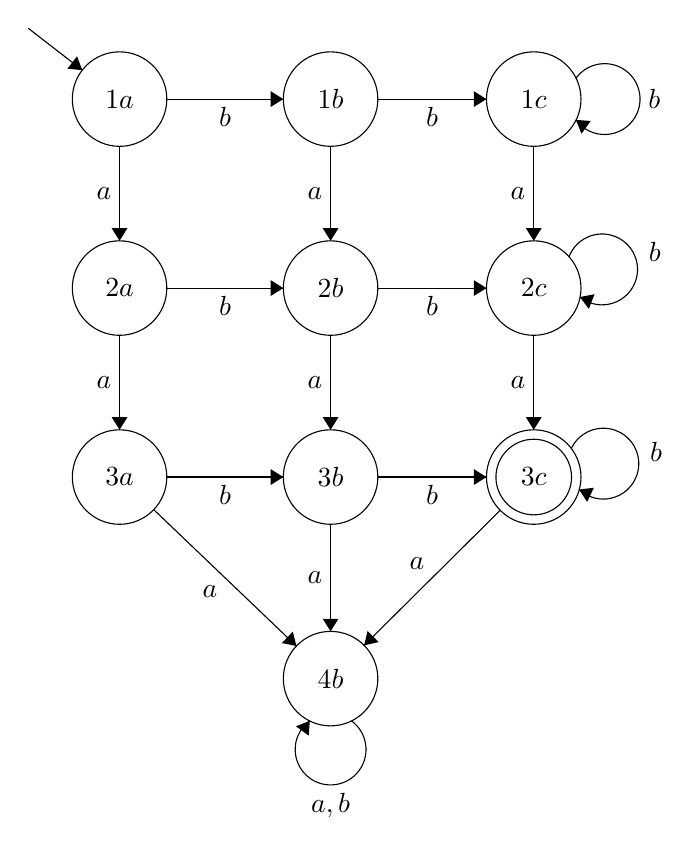
\begin{tikzpicture}[scale=0.2]
\tikzstyle{every node}+=[inner sep=0pt]
\draw [black] (7.4,-5.7) circle (3);
\draw (7.4,-5.7) node {$1a$};
\draw [black] (20.8,-5.7) circle (3);
\draw (20.8,-5.7) node {$1b$};
\draw [black] (33.7,-5.7) circle (3);
\draw (33.7,-5.7) node {$1c$};
\draw [black] (7.4,-17.7) circle (3);
\draw (7.4,-17.7) node {$2a$};
\draw [black] (20.8,-17.7) circle (3);
\draw (20.8,-17.7) node {$2b$};
\draw [black] (33.7,-17.7) circle (3);
\draw (33.7,-17.7) node {$2c$};
\draw [black] (7.4,-29.7) circle (3);
\draw (7.4,-29.7) node {$3a$};
\draw [black] (20.8,-29.7) circle (3);
\draw (20.8,-29.7) node {$3b$};
\draw [black] (33.7,-29.7) circle (3);
\draw (33.7,-29.7) node {$3c$};
\draw [black] (33.7,-29.7) circle (2.4);
\draw [black] (20.8,-42.5) circle (3);
\draw (20.8,-42.5) node {$4b$};
\draw [black] (1.6,-1.2) -- (5.03,-3.86);
\fill [black] (5.03,-3.86) -- (4.7,-2.98) -- (4.09,-3.77);
\draw [black] (10.4,-5.7) -- (17.8,-5.7);
\fill [black] (17.8,-5.7) -- (17,-5.2) -- (17,-6.2);
\draw (14.1,-6.2) node [below] {$b$};
\draw [black] (23.8,-5.7) -- (30.7,-5.7);
\fill [black] (30.7,-5.7) -- (29.9,-5.2) -- (29.9,-6.2);
\draw (27.25,-6.2) node [below] {$b$};
\draw [black] (7.4,-8.7) -- (7.4,-14.7);
\fill [black] (7.4,-14.7) -- (7.9,-13.9) -- (6.9,-13.9);
\draw (6.9,-11.7) node [left] {$a$};
\draw [black] (10.4,-17.7) -- (17.8,-17.7);
\fill [black] (17.8,-17.7) -- (17,-17.2) -- (17,-18.2);
\draw (14.1,-18.2) node [below] {$b$};
\draw [black] (20.8,-8.7) -- (20.8,-14.7);
\fill [black] (20.8,-14.7) -- (21.3,-13.9) -- (20.3,-13.9);
\draw (20.3,-11.7) node [left] {$a$};
\draw [black] (23.8,-17.7) -- (30.7,-17.7);
\fill [black] (30.7,-17.7) -- (29.9,-17.2) -- (29.9,-18.2);
\draw (27.25,-18.2) node [below] {$b$};
\draw [black] (33.7,-8.7) -- (33.7,-14.7);
\fill [black] (33.7,-14.7) -- (34.2,-13.9) -- (33.2,-13.9);
\draw (33.2,-11.7) node [left] {$a$};
\draw [black] (7.4,-20.7) -- (7.4,-26.7);
\fill [black] (7.4,-26.7) -- (7.9,-25.9) -- (6.9,-25.9);
\draw (6.9,-23.7) node [left] {$a$};
\draw [black] (20.8,-20.7) -- (20.8,-26.7);
\fill [black] (20.8,-26.7) -- (21.3,-25.9) -- (20.3,-25.9);
\draw (20.3,-23.7) node [left] {$a$};
\draw [black] (33.7,-20.7) -- (33.7,-26.7);
\fill [black] (33.7,-26.7) -- (34.2,-25.9) -- (33.2,-25.9);
\draw (33.2,-23.7) node [left] {$a$};
\draw [black] (10.4,-29.7) -- (17.8,-29.7);
\fill [black] (17.8,-29.7) -- (17,-29.2) -- (17,-30.2);
\draw (14.1,-30.2) node [below] {$b$};
\draw [black] (23.8,-29.7) -- (30.7,-29.7);
\fill [black] (30.7,-29.7) -- (29.9,-29.2) -- (29.9,-30.2);
\draw (27.25,-30.2) node [below] {$b$};
\draw [black] (20.8,-32.7) -- (20.8,-39.5);
\fill [black] (20.8,-39.5) -- (21.3,-38.7) -- (20.3,-38.7);
\draw (20.3,-36.1) node [left] {$a$};
\draw [black] (9.57,-31.77) -- (18.63,-40.43);
\fill [black] (18.63,-40.43) -- (18.4,-39.51) -- (17.71,-40.24);
\draw (13.14,-36.58) node [below] {$a$};
\draw [black] (31.57,-31.81) -- (22.93,-40.39);
\fill [black] (22.93,-40.39) -- (23.85,-40.18) -- (23.15,-39.47);
\draw (26.28,-35.62) node [above] {$a$};
\draw [black] (36.082,-27.895) arc (154.88553:-133.11447:2.25);
\draw (41.06,-28.13) node [right] {$b$};
\fill [black] (36.58,-30.49) -- (37.09,-31.28) -- (37.52,-30.38);
\draw [black] (22.123,-45.18) arc (54:-234:2.25);
\draw (20.8,-49.75) node [below] {$a,b$};
\fill [black] (19.48,-45.18) -- (18.6,-45.53) -- (19.41,-46.12);
\draw [black] (36.38,-4.377) arc (144:-144:2.25);
\draw (40.95,-5.7) node [right] {$b$};
\fill [black] (36.38,-7.02) -- (36.73,-7.9) -- (37.32,-7.09);
\draw [black] (35.937,-15.719) arc (159.25512:-128.74488:2.25);
\draw (40.98,-15.4) node [right] {$b$};
\fill [black] (36.63,-18.27) -- (37.2,-19.02) -- (37.56,-18.09);
\end{tikzpicture}
\end{center}

\textbf{c}

\begin{center}
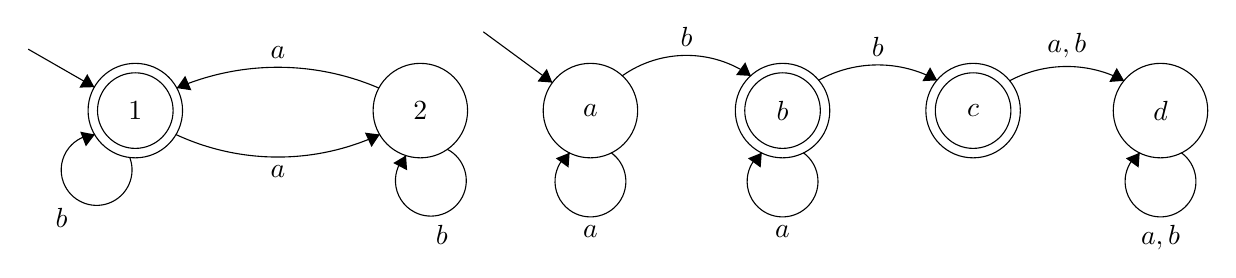
\begin{tikzpicture}[scale=0.2]
\tikzstyle{every node}+=[inner sep=0pt]
\draw [black] (10.1,-7.1) circle (3);
\draw (10.1,-7.1) node {$1$};
\draw [black] (10.1,-7.1) circle (2.4);
\draw [black] (28.2,-7.1) circle (3);
\draw (28.2,-7.1) node {$2$};
\draw [black] (39,-7.1) circle (3);
\draw (39,-7.1) node {$a$};
\draw [black] (51.2,-7.1) circle (3);
\draw (51.2,-7.1) node {$b$};
\draw [black] (51.2,-7.1) circle (2.4);
\draw [black] (63.3,-7.1) circle (3);
\draw (63.3,-7.1) node {$c$};
\draw [black] (63.3,-7.1) circle (2.4);
\draw [black] (75.2,-7.1) circle (3);
\draw (75.2,-7.1) node {$d$};
\draw [black] (3.3,-3.2) -- (7.5,-5.61);
\fill [black] (7.5,-5.61) -- (7.05,-4.78) -- (6.55,-5.64);
\draw [black] (25.62,-8.621) arc (-65.08079:-114.91921:15.355);
\fill [black] (25.62,-8.62) -- (24.68,-8.5) -- (25.1,-9.41);
\draw (19.15,-10.55) node [below] {$a$};
\draw [black] (12.732,-5.669) arc (113.25012:66.74988:16.259);
\fill [black] (12.73,-5.67) -- (13.66,-5.81) -- (13.27,-4.89);
\draw (19.15,-3.85) node [above] {$a$};
\draw [black] (32.2,-2.1) -- (36.58,-5.32);
\fill [black] (36.58,-5.32) -- (36.23,-4.45) -- (35.64,-5.25);
\draw [black] (41.007,-4.901) arc (125.43267:54.56733:7.059);
\fill [black] (49.19,-4.9) -- (48.83,-4.03) -- (48.25,-4.84);
\draw (45.1,-3.09) node [above] {$b$};
\draw [black] (53.479,-5.177) arc (119.07851:60.92149:7.76);
\fill [black] (61.02,-5.18) -- (60.57,-4.35) -- (60.08,-5.23);
\draw (57.25,-3.7) node [above] {$b$};
\draw [black] (65.607,-5.212) arc (118.16267:61.83733:7.719);
\fill [black] (72.89,-5.21) -- (72.42,-4.39) -- (71.95,-5.28);
\draw (69.25,-3.8) node [above] {$a,b$};
\draw [black] (40.323,-9.78) arc (54:-234:2.25);
\draw (39,-14.35) node [below] {$a$};
\fill [black] (37.68,-9.78) -- (36.8,-10.13) -- (37.61,-10.72);
\draw [black] (52.523,-9.78) arc (54:-234:2.25);
\draw (51.2,-14.35) node [below] {$a$};
\fill [black] (49.88,-9.78) -- (49,-10.13) -- (49.81,-10.72);
\draw [black] (76.523,-9.78) arc (54:-234:2.25);
\draw (75.2,-14.35) node [below] {$a,b$};
\fill [black] (73.88,-9.78) -- (73,-10.13) -- (73.81,-10.72);
\draw [black] (9.744,-10.067) arc (20.88866:-267.11134:2.25);
\draw (5.41,-13.25) node [below] {$b$};
\fill [black] (7.53,-8.62) -- (6.6,-8.44) -- (6.96,-9.37);
\draw [black] (29.905,-9.554) arc (62.53077:-225.46923:2.25);
\draw (29.57,-14.37) node [below] {$b$};
\fill [black] (27.29,-9.95) -- (26.48,-10.43) -- (27.36,-10.89);
\end{tikzpicture}
\end{center}

\begin{center}
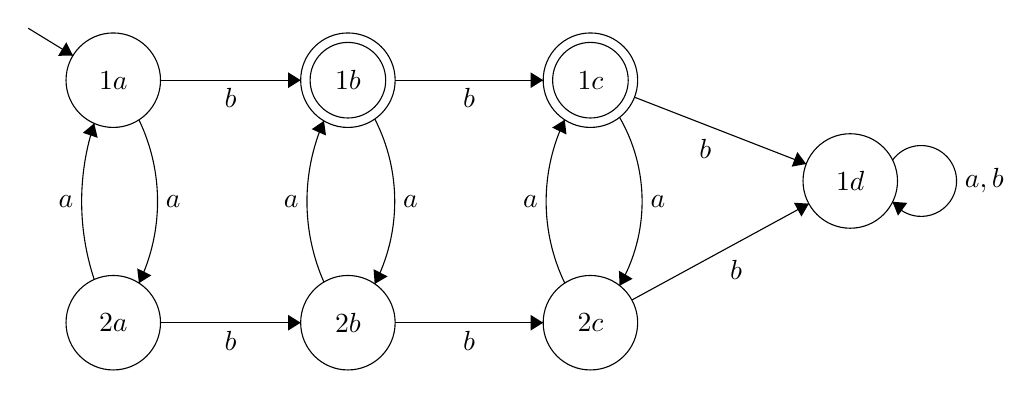
\begin{tikzpicture}[scale=0.2]
\tikzstyle{every node}+=[inner sep=0pt]
\draw [black] (8.1,-6.6) circle (3);
\draw (8.1,-6.6) node {$1a$};
\draw [black] (8.1,-22) circle (3);
\draw (8.1,-22) node {$2a$};
\draw [black] (23,-6.6) circle (3);
\draw (23,-6.6) node {$1b$};
\draw [black] (23,-6.6) circle (2.4);
\draw [black] (23,-22) circle (3);
\draw (23,-22) node {$2b$};
\draw [black] (38.4,-6.6) circle (3);
\draw (38.4,-6.6) node {$1c$};
\draw [black] (38.4,-6.6) circle (2.4);
\draw [black] (38.4,-22) circle (3);
\draw (38.4,-22) node {$2c$};
\draw [black] (54.9,-13) circle (3);
\draw (54.9,-13) node {$1d$};
\draw [black] (2.7,-3.3) -- (5.54,-5.04);
\fill [black] (5.54,-5.04) -- (5.12,-4.19) -- (4.6,-5.05);
\draw [black] (9.727,-9.111) arc (25.73953:-25.73953:11.948);
\fill [black] (9.73,-19.49) -- (10.52,-18.99) -- (9.62,-18.55);
\draw (11.41,-14.3) node [right] {$a$};
\draw [black] (24.704,-9.058) arc (27.23117:-27.23117:11.455);
\fill [black] (24.7,-19.54) -- (25.52,-19.06) -- (24.63,-18.6);
\draw (26.47,-14.3) node [right] {$a$};
\draw [black] (40.246,-8.952) arc (30.0658:-30.0658:10.674);
\fill [black] (40.25,-19.65) -- (41.08,-19.21) -- (40.21,-18.7);
\draw (42.18,-14.3) node [right] {$a$};
\draw [black] (6.892,-19.259) arc (-161.66604:-198.33396:15.765);
\fill [black] (6.89,-9.34) -- (6.17,-9.94) -- (7.11,-10.26);
\draw (5.59,-14.3) node [left] {$a$};
\draw [black] (21.478,-19.423) arc (-156.21298:-203.78702:12.7);
\fill [black] (21.48,-9.18) -- (20.7,-9.71) -- (21.61,-10.11);
\draw (19.9,-14.3) node [left] {$a$};
\draw [black] (36.773,-19.489) arc (-154.24867:-205.75133:11.944);
\fill [black] (36.77,-9.11) -- (35.97,-9.61) -- (36.88,-10.05);
\draw (35.09,-14.3) node [left] {$a$};
\draw [black] (11.1,-6.6) -- (20,-6.6);
\fill [black] (20,-6.6) -- (19.2,-6.1) -- (19.2,-7.1);
\draw (15.55,-7.1) node [below] {$b$};
\draw [black] (11.1,-22) -- (20,-22);
\fill [black] (20,-22) -- (19.2,-21.5) -- (19.2,-22.5);
\draw (15.55,-22.5) node [below] {$b$};
\draw [black] (26,-6.6) -- (35.4,-6.6);
\fill [black] (35.4,-6.6) -- (34.6,-6.1) -- (34.6,-7.1);
\draw (30.7,-7.1) node [below] {$b$};
\draw [black] (26,-22) -- (35.4,-22);
\fill [black] (35.4,-22) -- (34.6,-21.5) -- (34.6,-22.5);
\draw (30.7,-22.5) node [below] {$b$};
\draw [black] (41.2,-7.68) -- (52.1,-11.92);
\fill [black] (52.1,-11.92) -- (51.54,-11.16) -- (51.18,-12.09);
\draw (45.7,-10.32) node [below] {$b$};
\draw [black] (41.03,-20.56) -- (52.27,-14.44);
\fill [black] (52.27,-14.44) -- (51.32,-14.38) -- (51.8,-15.26);
\draw (47.65,-18) node [below] {$b$};
\draw [black] (57.58,-11.677) arc (144:-144:2.25);
\draw (62.15,-13) node [right] {$a,b$};
\fill [black] (57.58,-14.32) -- (57.93,-15.2) -- (58.52,-14.39);
\end{tikzpicture}
\end{center}

\pagebreak

\textbf{d}
\begin{center}
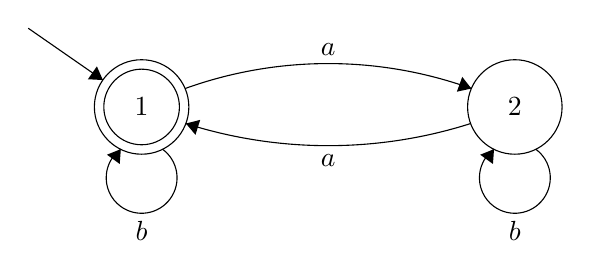
\begin{tikzpicture}[scale=0.2]
\tikzstyle{every node}+=[inner sep=0pt]
\draw [black] (8.6,-6.7) circle (3);
\draw (8.6,-6.7) node {$1$};
\draw [black] (8.6,-6.7) circle (2.4);
\draw [black] (32.3,-6.7) circle (3);
\draw (32.3,-6.7) node {$2$};
\draw [black] (11.36,-5.529) arc (109.79245:70.20755:26.844);
\fill [black] (29.54,-5.53) -- (28.96,-4.79) -- (28.62,-5.73);
\draw (20.45,-3.44) node [above] {$a$};
\draw [black] (29.492,-7.753) arc (-72.33607:-107.66393:29.799);
\fill [black] (11.41,-7.75) -- (12.02,-8.47) -- (12.32,-7.52);
\draw (20.45,-9.66) node [below] {$a$};
\draw [black] (1.4,-1.7) -- (6.14,-4.99);
\fill [black] (6.14,-4.99) -- (5.76,-4.12) -- (5.19,-4.94);
\draw [black] (9.923,-9.38) arc (54:-234:2.25);
\draw (8.6,-13.95) node [below] {$b$};
\fill [black] (7.28,-9.38) -- (6.4,-9.73) -- (7.21,-10.32);
\draw [black] (33.623,-9.38) arc (54:-234:2.25);
\draw (32.3,-13.95) node [below] {$b$};
\fill [black] (30.98,-9.38) -- (30.1,-9.73) -- (30.91,-10.32);
\end{tikzpicture}
\end{center}


\begin{center}
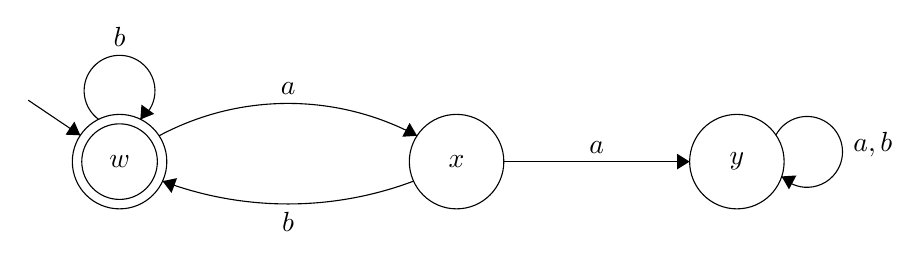
\begin{tikzpicture}[scale=0.2]
\tikzstyle{every node}+=[inner sep=0pt]
\draw [black] (10,-10.9) circle (3);
\draw (10,-10.9) node {$w$};
\draw [black] (10,-10.9) circle (2.4);
\draw [black] (31.4,-10.9) circle (3);
\draw (31.4,-10.9) node {$x$};
\draw [black] (49.2,-10.9) circle (3);
\draw (49.2,-10.9) node {$y$};
\draw [black] (4.2,-7) -- (7.51,-9.23);
\fill [black] (7.51,-9.23) -- (7.13,-8.36) -- (6.57,-9.19);
\draw [black] (12.508,-9.261) arc (118.19767:61.80233:17.336);
\fill [black] (28.89,-9.26) -- (28.42,-8.44) -- (27.95,-9.32);
\draw (20.7,-6.7) node [above] {$a$};
\draw [black] (34.4,-10.9) -- (46.2,-10.9);
\fill [black] (46.2,-10.9) -- (45.4,-10.4) -- (45.4,-11.4);
\draw (40.3,-10.4) node [above] {$a$};
\draw [black] (51.673,-9.222) arc (151.88957:-136.11043:2.25);
\draw (56.57,-9.81) node [right] {$a,b$};
\fill [black] (52.04,-11.84) -- (52.51,-12.66) -- (52.98,-11.78);
\draw [black] (8.677,-8.22) arc (234:-54:2.25);
\draw (10,-3.65) node [above] {$b$};
\fill [black] (11.32,-8.22) -- (12.2,-7.87) -- (11.39,-7.28);
\draw [black] (28.67,-12.139) arc (-69.38456:-110.61544:22.637);
\fill [black] (12.73,-12.14) -- (13.3,-12.89) -- (13.65,-11.95);
\draw (20.7,-14.09) node [below] {$b$};
\end{tikzpicture}
\end{center}

\begin{center}
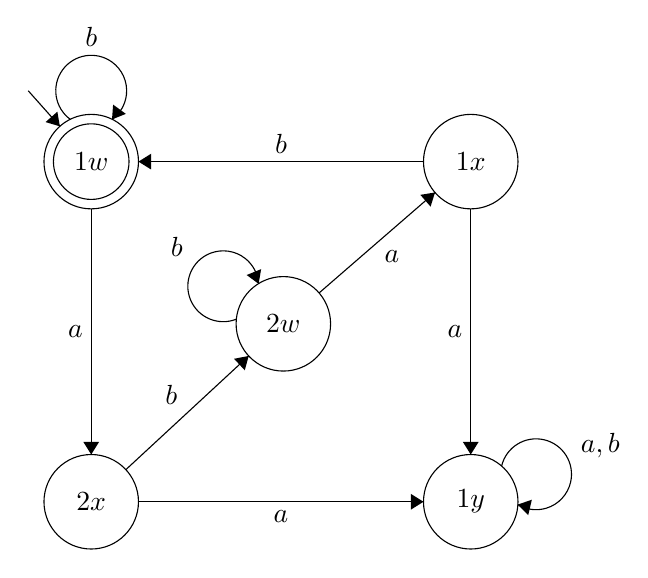
\begin{tikzpicture}[scale=0.2]
\tikzstyle{every node}+=[inner sep=0pt]
\draw [black] (9.2,-31) circle (3);
\draw (9.2,-31) node {$2x$};
\draw [black] (33.3,-31) circle (3);
\draw (33.3,-31) node {$1y$};
\draw [black] (21.4,-19.7) circle (3);
\draw (21.4,-19.7) node {$2w$};
\draw [black] (33.3,-9.4) circle (3);
\draw (33.3,-9.4) node {$1x$};
\draw [black] (9.2,-9.4) circle (3);
\draw (9.2,-9.4) node {$1w$};
\draw [black] (9.2,-9.4) circle (2.4);
\draw [black] (12.2,-31) -- (30.3,-31);
\fill [black] (30.3,-31) -- (29.5,-30.5) -- (29.5,-31.5);
\draw (21.25,-31.5) node [below] {$a$};
\draw [black] (35.257,-28.741) arc (166.83365:-121.16635:2.25);
\draw (40.26,-27.44) node [right] {$a,b$};
\fill [black] (36.28,-31.18) -- (36.95,-31.85) -- (37.18,-30.87);
\draw [black] (11.4,-28.96) -- (19.2,-21.74);
\fill [black] (19.2,-21.74) -- (18.27,-21.92) -- (18.95,-22.65);
\draw (14.28,-24.86) node [above] {$b$};
\draw [black] (18.427,-19.401) arc (291.99248:3.99248:2.25);
\draw (15.05,-14.83) node [left] {$b$};
\fill [black] (19.83,-17.16) -- (19.99,-16.23) -- (19.07,-16.6);
\draw [black] (23.67,-17.74) -- (31.03,-11.36);
\fill [black] (31.03,-11.36) -- (30.1,-11.51) -- (30.75,-12.26);
\draw (28.3,-15.04) node [below] {$a$};
\draw [black] (33.3,-12.4) -- (33.3,-28);
\fill [black] (33.3,-28) -- (33.8,-27.2) -- (32.8,-27.2);
\draw (32.8,-20.2) node [left] {$a$};
\draw [black] (5.2,-4.9) -- (7.21,-7.16);
\fill [black] (7.21,-7.16) -- (7.05,-6.23) -- (6.3,-6.89);
\draw [black] (7.877,-6.72) arc (234:-54:2.25);
\draw (9.2,-2.15) node [above] {$b$};
\fill [black] (10.52,-6.72) -- (11.4,-6.37) -- (10.59,-5.78);
\draw [black] (9.2,-12.4) -- (9.2,-28);
\fill [black] (9.2,-28) -- (9.7,-27.2) -- (8.7,-27.2);
\draw (8.7,-20.2) node [left] {$a$};
\draw [black] (30.3,-9.4) -- (12.2,-9.4);
\fill [black] (12.2,-9.4) -- (13,-9.9) -- (13,-8.9);
\draw (21.25,-8.9) node [above] {$b$};
\end{tikzpicture}
\end{center}

\textbf{e}
\begin{center}
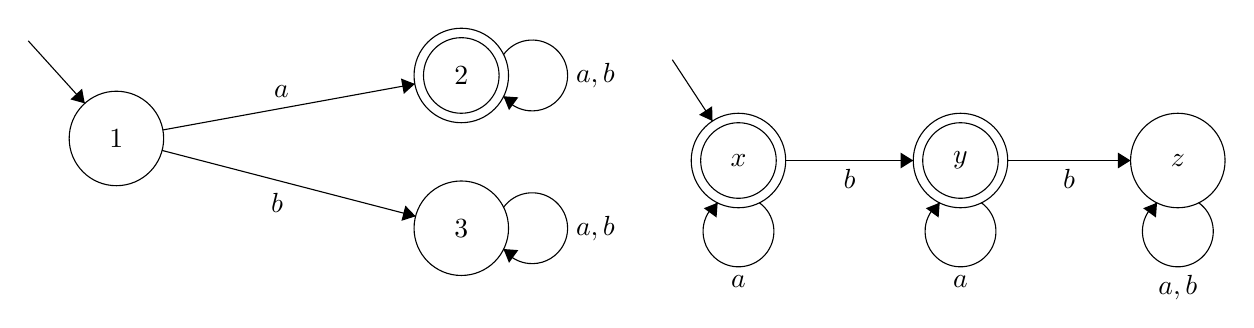
\begin{tikzpicture}[scale=0.2]
\tikzstyle{every node}+=[inner sep=0pt]
\draw [black] (8.5,-8.2) circle (3);
\draw (8.5,-8.2) node {$1$};
\draw [black] (30.4,-4.2) circle (3);
\draw (30.4,-4.2) node {$2$};
\draw [black] (30.4,-4.2) circle (2.4);
\draw [black] (30.4,-13.9) circle (3);
\draw (30.4,-13.9) node {$3$};
\draw [black] (48,-9.6) circle (3);
\draw (48,-9.6) node {$x$};
\draw [black] (48,-9.6) circle (2.4);
\draw [black] (62.1,-9.6) circle (3);
\draw (62.1,-9.6) node {$y$};
\draw [black] (62.1,-9.6) circle (2.4);
\draw [black] (75.9,-9.6) circle (3);
\draw (75.9,-9.6) node {$z$};
\draw [black] (11.45,-7.66) -- (27.45,-4.74);
\fill [black] (27.45,-4.74) -- (26.57,-4.39) -- (26.75,-5.37);
\draw (18.98,-5.61) node [above] {$a$};
\draw [black] (33.08,-2.877) arc (144:-144:2.25);
\draw (37.65,-4.2) node [right] {$a,b$};
\fill [black] (33.08,-5.52) -- (33.43,-6.4) -- (34.02,-5.59);
\draw [black] (11.4,-8.96) -- (27.5,-13.14);
\fill [black] (27.5,-13.14) -- (26.85,-12.46) -- (26.6,-13.43);
\draw (18.7,-11.62) node [below] {$b$};
\draw [black] (33.08,-12.577) arc (144:-144:2.25);
\draw (37.65,-13.9) node [right] {$a,b$};
\fill [black] (33.08,-15.22) -- (33.43,-16.1) -- (34.02,-15.29);
\draw [black] (2.9,-2) -- (6.49,-5.97);
\fill [black] (6.49,-5.97) -- (6.32,-5.04) -- (5.58,-5.72);
\draw [black] (43.8,-3.2) -- (46.35,-7.09);
\fill [black] (46.35,-7.09) -- (46.33,-6.15) -- (45.5,-6.7);
\draw [black] (49.323,-12.28) arc (54:-234:2.25);
\draw (48,-16.85) node [below] {$a$};
\fill [black] (46.68,-12.28) -- (45.8,-12.63) -- (46.61,-13.22);
\draw [black] (51,-9.6) -- (59.1,-9.6);
\fill [black] (59.1,-9.6) -- (58.3,-9.1) -- (58.3,-10.1);
\draw (55.05,-10.1) node [below] {$b$};
\draw [black] (63.423,-12.28) arc (54:-234:2.25);
\draw (62.1,-16.85) node [below] {$a$};
\fill [black] (60.78,-12.28) -- (59.9,-12.63) -- (60.71,-13.22);
\draw [black] (65.1,-9.6) -- (72.9,-9.6);
\fill [black] (72.9,-9.6) -- (72.1,-9.1) -- (72.1,-10.1);
\draw (69,-10.1) node [below] {$b$};
\draw [black] (77.223,-12.28) arc (54:-234:2.25);
\draw (75.9,-16.85) node [below] {$a,b$};
\fill [black] (74.58,-12.28) -- (73.7,-12.63) -- (74.51,-13.22);
\end{tikzpicture}
\end{center}

\begin{center}
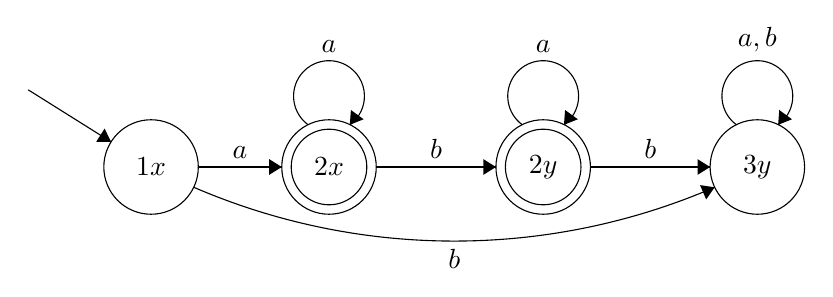
\begin{tikzpicture}[scale=0.2]
\tikzstyle{every node}+=[inner sep=0pt]
\draw [black] (9.2,-9.2) circle (3);
\draw (9.2,-9.2) node {$1x$};
\draw [black] (20.5,-9.2) circle (3);
\draw (20.5,-9.2) node {$2x$};
\draw [black] (20.5,-9.2) circle (2.4);
\draw [black] (34.1,-9.2) circle (3);
\draw (34.1,-9.2) node {$2y$};
\draw [black] (34.1,-9.2) circle (2.4);
\draw [black] (47.7,-9.2) circle (3);
\draw (47.7,-9.2) node {$3y$};
\draw [black] (1.4,-4.3) -- (6.66,-7.6);
\fill [black] (6.66,-7.6) -- (6.25,-6.76) -- (5.72,-7.6);
\draw [black] (12.2,-9.2) -- (17.5,-9.2);
\fill [black] (17.5,-9.2) -- (16.7,-8.7) -- (16.7,-9.7);
\draw (14.85,-8.7) node [above] {$a$};
\draw [black] (44.991,-10.487) arc (-66.64911:-113.35089:41.732);
\fill [black] (44.99,-10.49) -- (44.06,-10.35) -- (44.45,-11.26);
\draw (28.45,-14.41) node [below] {$b$};
\draw [black] (19.177,-6.52) arc (234:-54:2.25);
\draw (20.5,-1.95) node [above] {$a$};
\fill [black] (21.82,-6.52) -- (22.7,-6.17) -- (21.89,-5.58);
\draw [black] (23.5,-9.2) -- (31.1,-9.2);
\fill [black] (31.1,-9.2) -- (30.3,-8.7) -- (30.3,-9.7);
\draw (27.3,-8.7) node [above] {$b$};
\draw [black] (46.377,-6.52) arc (234:-54:2.25);
\draw (47.7,-1.95) node [above] {$a,b$};
\fill [black] (49.02,-6.52) -- (49.9,-6.17) -- (49.09,-5.58);
\draw [black] (32.777,-6.52) arc (234:-54:2.25);
\draw (34.1,-1.95) node [above] {$a$};
\fill [black] (35.42,-6.52) -- (36.3,-6.17) -- (35.49,-5.58);
\draw [black] (37.1,-9.2) -- (44.7,-9.2);
\fill [black] (44.7,-9.2) -- (43.9,-8.7) -- (43.9,-9.7);
\draw (40.9,-8.7) node [above] {$b$};
\end{tikzpicture}
\end{center}

\textbf{f}

\begin{center}
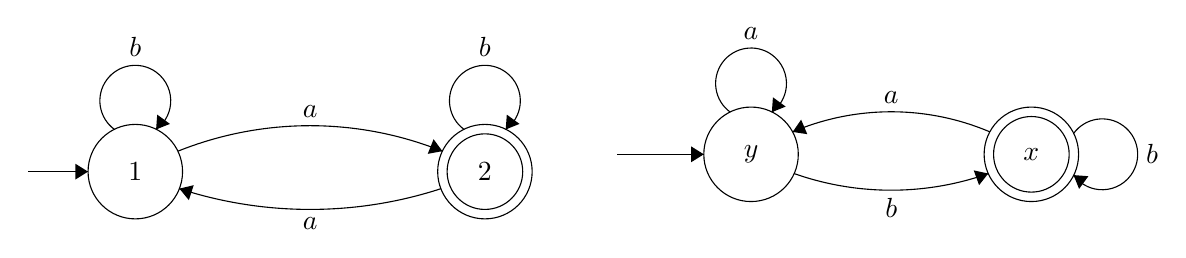
\begin{tikzpicture}[scale=0.2]
\tikzstyle{every node}+=[inner sep=0pt]
\draw [black] (8.3,-9.7) circle (3);
\draw (8.3,-9.7) node {$1$};
\draw [black] (30.5,-9.7) circle (3);
\draw (30.5,-9.7) node {$2$};
\draw [black] (30.5,-9.7) circle (2.4);
\draw [black] (47.4,-8.6) circle (3);
\draw (47.4,-8.6) node {$y$};
\draw [black] (65.2,-8.6) circle (3);
\draw (65.2,-8.6) node {$x$};
\draw [black] (65.2,-8.6) circle (2.4);
\draw [black] (1.5,-9.7) -- (5.3,-9.7);
\fill [black] (5.3,-9.7) -- (4.5,-9.2) -- (4.5,-10.2);
\draw [black] (11.002,-8.402) arc (111.8419:68.1581:22.571);
\fill [black] (27.8,-8.4) -- (27.24,-7.64) -- (26.87,-8.57);
\draw (19.4,-6.28) node [above] {$a$};
\draw [black] (27.705,-10.784) arc (-71.99636:-108.00364:26.869);
\fill [black] (11.1,-10.78) -- (11.7,-11.51) -- (12.01,-10.56);
\draw (19.4,-12.6) node [below] {$a$};
\draw [black] (6.977,-7.02) arc (234:-54:2.25);
\draw (8.3,-2.45) node [above] {$b$};
\fill [black] (9.62,-7.02) -- (10.5,-6.67) -- (9.69,-6.08);
\draw [black] (29.177,-7.02) arc (234:-54:2.25);
\draw (30.5,-2.45) node [above] {$b$};
\fill [black] (31.82,-7.02) -- (32.7,-6.67) -- (31.89,-6.08);
\draw [black] (62.464,-9.823) arc (-70.56342:-109.43658:18.524);
\fill [black] (62.46,-9.82) -- (61.54,-9.62) -- (61.88,-10.56);
\draw (56.3,-11.38) node [below] {$b$};
\draw [black] (67.88,-7.277) arc (144:-144:2.25);
\draw (72.45,-8.6) node [right] {$b$};
\fill [black] (67.88,-9.92) -- (68.23,-10.8) -- (68.82,-9.99);
\draw [black] (50.035,-7.175) arc (113.03259:66.96741:16.012);
\fill [black] (50.04,-7.18) -- (50.97,-7.32) -- (50.58,-6.4);
\draw (56.3,-5.4) node [above] {$a$};
\draw [black] (46.077,-5.92) arc (234:-54:2.25);
\draw (47.4,-1.35) node [above] {$a$};
\fill [black] (48.72,-5.92) -- (49.6,-5.57) -- (48.79,-4.98);
\draw [black] (38.9,-8.6) -- (44.4,-8.6);
\fill [black] (44.4,-8.6) -- (43.6,-8.1) -- (43.6,-9.1);
\end{tikzpicture}
\end{center}

\begin{center}
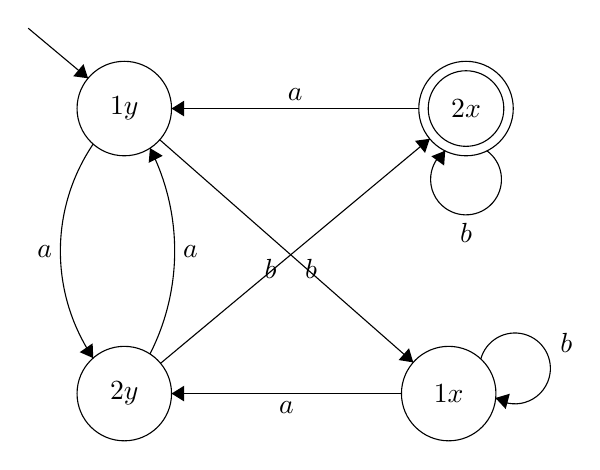
\begin{tikzpicture}[scale=0.2]
\tikzstyle{every node}+=[inner sep=0pt]
\draw [black] (13,-8.5) circle (3);
\draw (13,-8.5) node {$1y$};
\draw [black] (13,-26.6) circle (3);
\draw (13,-26.6) node {$2y$};
\draw [black] (33.6,-26.6) circle (3);
\draw (33.6,-26.6) node {$1x$};
\draw [black] (34.7,-8.5) circle (3);
\draw (34.7,-8.5) node {$2x$};
\draw [black] (34.7,-8.5) circle (2.4);
\draw [black] (6.9,-3.4) -- (10.7,-6.58);
\fill [black] (10.7,-6.58) -- (10.41,-5.68) -- (9.76,-6.45);
\draw [black] (11.028,-24.349) arc (-145.86932:-214.13068:12.118);
\fill [black] (11.03,-24.35) -- (10.99,-23.41) -- (10.17,-23.97);
\draw (8.44,-17.55) node [left] {$a$};
\draw [black] (15.25,-10.48) -- (31.35,-24.62);
\fill [black] (31.35,-24.62) -- (31.08,-23.72) -- (30.42,-24.47);
\draw (22.29,-18.04) node [below] {$b$};
\draw [black] (30.6,-26.6) -- (16,-26.6);
\fill [black] (16,-26.6) -- (16.8,-27.1) -- (16.8,-26.1);
\draw (23.3,-27.1) node [below] {$a$};
\draw [black] (35.636,-24.412) arc (164.79632:-123.20368:2.25);
\draw (40.66,-23.37) node [right] {$b$};
\fill [black] (36.57,-26.88) -- (37.22,-27.58) -- (37.48,-26.61);
\draw [black] (14.63,-11.012) arc (27.0074:-27.0074:14.397);
\fill [black] (14.63,-11.01) -- (14.55,-11.95) -- (15.44,-11.5);
\draw (16.7,-17.55) node [right] {$a$};
\draw [black] (15.3,-24.68) -- (32.4,-10.42);
\fill [black] (32.4,-10.42) -- (31.46,-10.55) -- (32.1,-11.32);
\draw (24.86,-18.04) node [below] {$b$};
\draw [black] (36.023,-11.18) arc (54:-234:2.25);
\draw (34.7,-15.75) node [below] {$b$};
\fill [black] (33.38,-11.18) -- (32.5,-11.53) -- (33.31,-12.12);
\draw [black] (31.7,-8.5) -- (16,-8.5);
\fill [black] (16,-8.5) -- (16.8,-9) -- (16.8,-8);
\draw (23.85,-8) node [above] {$a$};
\end{tikzpicture}
\end{center}

\end{homeworkProblem}


\begin{homeworkProblem}
\textbf{1.6f}
\begin{center}
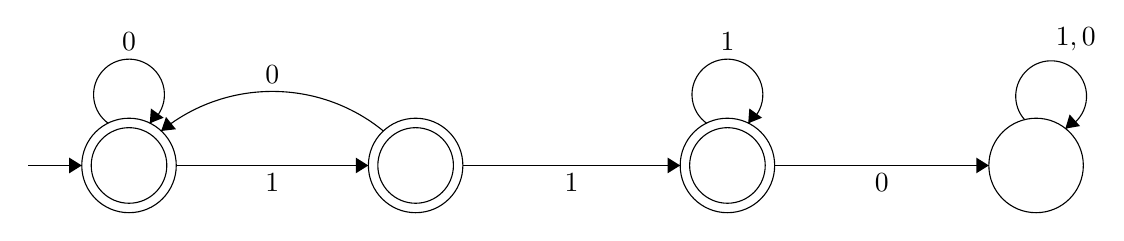
\begin{tikzpicture}[scale=0.2]
\tikzstyle{every node}+=[inner sep=0pt]
\draw [black] (10.6,-11.7) circle (3);
\draw [black] (10.6,-11.7) circle (2.4);
\draw [black] (28.8,-11.7) circle (3);
\draw [black] (28.8,-11.7) circle (2.4);
\draw [black] (48.6,-11.7) circle (3);
\draw [black] (48.6,-11.7) circle (2.4);
\draw [black] (68.2,-11.7) circle (3);
\draw [black] (4.2,-11.7) -- (7.6,-11.7);
\fill [black] (7.6,-11.7) -- (6.8,-11.2) -- (6.8,-12.2);
\draw [black] (13.6,-11.7) -- (25.8,-11.7);
\fill [black] (25.8,-11.7) -- (25,-11.2) -- (25,-12.2);
\draw (19.7,-12.2) node [below] {$1$};
\draw [black] (31.8,-11.7) -- (45.6,-11.7);
\fill [black] (45.6,-11.7) -- (44.8,-11.2) -- (44.8,-12.2);
\draw (38.7,-12.2) node [below] {$1$};
\draw [black] (51.6,-11.7) -- (65.2,-11.7);
\fill [black] (65.2,-11.7) -- (64.4,-11.2) -- (64.4,-12.2);
\draw (58.4,-12.2) node [below] {$0$};
\draw [black] (9.277,-9.02) arc (234:-54:2.25);
\draw (10.6,-4.45) node [above] {$0$};
\fill [black] (11.92,-9.02) -- (12.8,-8.67) -- (11.99,-8.08);
\draw [black] (12.642,-9.514) arc (129.24296:50.75704:11.157);
\fill [black] (12.64,-9.51) -- (13.58,-9.4) -- (12.95,-8.62);
\draw (19.7,-6.5) node [above] {$0$};
\draw [black] (67.477,-8.801) arc (221.73523:-66.26477:2.25);
\draw (70.72,-4.46) node [above] {$1,0$};
\fill [black] (70.06,-9.36) -- (70.99,-9.2) -- (70.33,-8.46);
\draw [black] (47.277,-9.02) arc (234:-54:2.25);
\draw (48.6,-4.45) node [above] {$1$};
\fill [black] (49.92,-9.02) -- (50.8,-8.67) -- (49.99,-8.08);
\end{tikzpicture}
\end{center}
\end{homeworkProblem}

\begin{homeworkProblem}
\textbf{1.6i}
\begin{center}
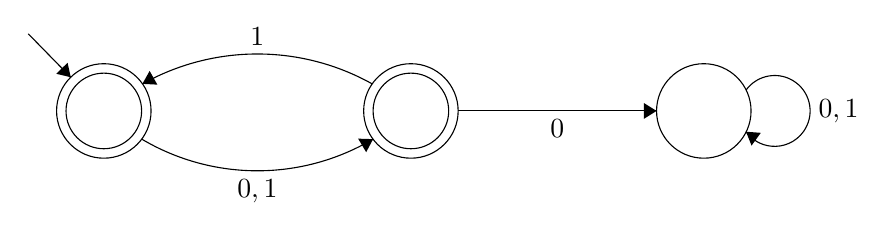
\begin{tikzpicture}[scale=0.2]
\tikzstyle{every node}+=[inner sep=0pt]
\draw [black] (10.4,-7.9) circle (3);
\draw [black] (10.4,-7.9) circle (2.4);
\draw [black] (29.9,-7.9) circle (3);
\draw [black] (29.9,-7.9) circle (2.4);
\draw [black] (48.5,-7.9) circle (3);
\draw [black] (5.6,-3) -- (8.3,-5.76);
\fill [black] (8.3,-5.76) -- (8.1,-4.84) -- (7.38,-5.54);
\draw [black] (27.497,-9.687) arc (-59.34009:-120.65991:14.407);
\fill [black] (27.5,-9.69) -- (26.55,-9.66) -- (27.06,-10.52);
\draw (20.15,-12.2) node [below] {$0,1$};
\draw [black] (12.854,-6.184) arc (119.21681:60.78319:14.947);
\fill [black] (12.85,-6.18) -- (13.8,-6.23) -- (13.31,-5.36);
\draw (20.15,-3.78) node [above] {$1$};
\draw [black] (32.9,-7.9) -- (45.5,-7.9);
\fill [black] (45.5,-7.9) -- (44.7,-7.4) -- (44.7,-8.4);
\draw (39.2,-8.4) node [below] {$0$};
\draw [black] (51.18,-6.577) arc (144:-144:2.25);
\draw (55.75,-7.9) node [right] {$0,1$};
\fill [black] (51.18,-9.22) -- (51.53,-10.1) -- (52.12,-9.29);
\end{tikzpicture}
\end{center}

\end{homeworkProblem}

\pagebreak


\begin{homeworkProblem}


\textbf{1.7c}


\begin{center}
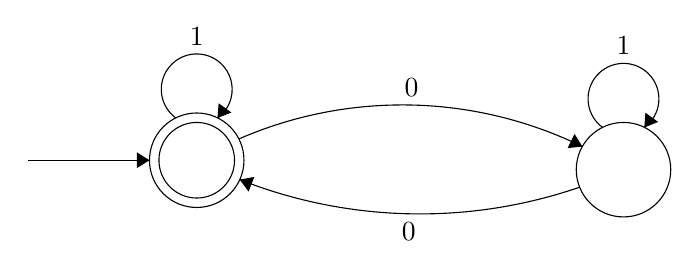
\begin{tikzpicture}[scale=0.2]
\tikzstyle{every node}+=[inner sep=0pt]
\draw [black] (17.1,-11.5) circle (3);
\draw [black] (17.1,-11.5) circle (2.4);
\draw [black] (44.2,-12.1) circle (3);
\draw [black] (6.4,-11.5) -- (14.1,-11.5);
\fill [black] (14.1,-11.5) -- (13.3,-11) -- (13.3,-12);
\draw [black] (19.776,-10.148) arc (113.51064:63.95269:26.026);
\fill [black] (41.59,-10.63) -- (41.09,-9.83) -- (40.65,-10.73);
\draw (30.74,-7.47) node [above] {$0$};
\draw [black] (41.415,-13.212) arc (-70.99514:-111.54152:31.15);
\fill [black] (19.83,-12.73) -- (20.39,-13.49) -- (20.76,-12.56);
\draw (30.57,-15.42) node [below] {$0$};
\draw [black] (15.777,-8.82) arc (234:-54:2.25);
\draw (17.1,-4.25) node [above] {$1$};
\fill [black] (18.42,-8.82) -- (19.3,-8.47) -- (18.49,-7.88);
\draw [black] (42.877,-9.42) arc (234:-54:2.25);
\draw (44.2,-4.85) node [above] {$1$};
\fill [black] (45.52,-9.42) -- (46.4,-9.07) -- (45.59,-8.48);
\end{tikzpicture}
\end{center}

\begin{center}
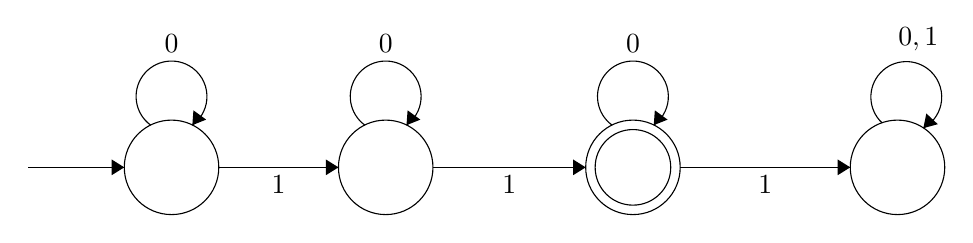
\begin{tikzpicture}[scale=0.2]
\tikzstyle{every node}+=[inner sep=0pt]
\draw [black] (10.5,-10.2) circle (3);
\draw [black] (24.1,-10.2) circle (3);
\draw [black] (39.8,-10.2) circle (3);
\draw [black] (39.8,-10.2) circle (2.4);
\draw [black] (56.6,-10.2) circle (3);
\draw [black] (1.4,-10.2) -- (7.5,-10.2);
\fill [black] (7.5,-10.2) -- (6.7,-9.7) -- (6.7,-10.7);
\draw [black] (13.5,-10.2) -- (21.1,-10.2);
\fill [black] (21.1,-10.2) -- (20.3,-9.7) -- (20.3,-10.7);
\draw (17.3,-10.7) node [below] {$1$};
\draw [black] (27.1,-10.2) -- (36.8,-10.2);
\fill [black] (36.8,-10.2) -- (36,-9.7) -- (36,-10.7);
\draw (31.95,-10.7) node [below] {$1$};
\draw [black] (9.177,-7.52) arc (234:-54:2.25);
\draw (10.5,-2.95) node [above] {$0$};
\fill [black] (11.82,-7.52) -- (12.7,-7.17) -- (11.89,-6.58);
\draw [black] (22.777,-7.52) arc (234:-54:2.25);
\draw (24.1,-2.95) node [above] {$0$};
\fill [black] (25.42,-7.52) -- (26.3,-7.17) -- (25.49,-6.58);
\draw [black] (38.477,-7.52) arc (234:-54:2.25);
\draw (39.8,-2.95) node [above] {$0$};
\fill [black] (41.12,-7.52) -- (42,-7.17) -- (41.19,-6.58);
\draw [black] (42.8,-10.2) -- (53.6,-10.2);
\fill [black] (53.6,-10.2) -- (52.8,-9.7) -- (52.8,-10.7);
\draw (48.2,-10.7) node [below] {$1$};
\draw [black] (55.62,-7.377) arc (226.87498:-61.12502:2.25);
\draw (57.92,-2.84) node [above] {$0,1$};
\fill [black] (58.24,-7.71) -- (59.16,-7.46) -- (58.43,-6.78);
\end{tikzpicture}
\end{center}


\begin{center}
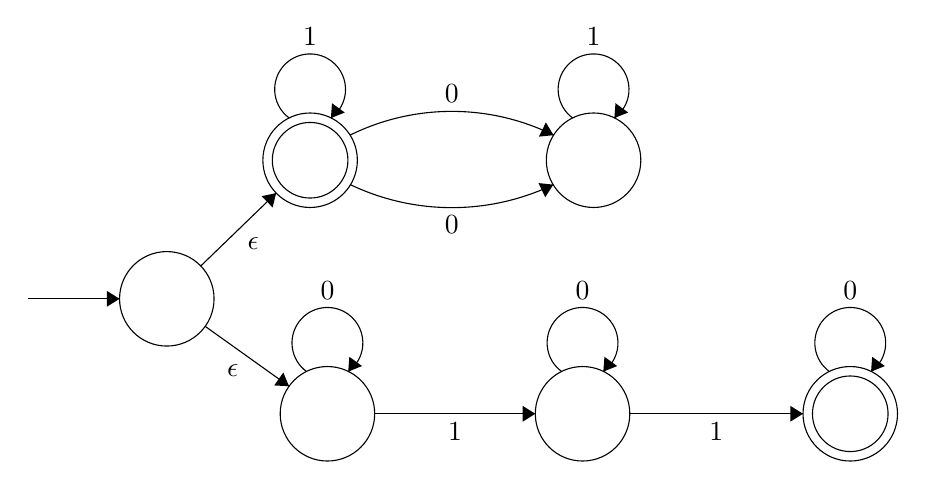
\begin{tikzpicture}[scale=0.2]
\tikzstyle{every node}+=[inner sep=0pt]
\draw [black] (10.1,-18.6) circle (3);
\draw [black] (19.2,-9.8) circle (3);
\draw [black] (19.2,-9.8) circle (2.4);
\draw [black] (37.2,-9.8) circle (3);
\draw [black] (20.3,-25.9) circle (3);
\draw [black] (36.5,-25.9) circle (3);
\draw [black] (53.5,-25.9) circle (3);
\draw [black] (53.5,-25.9) circle (2.4);
\draw [black] (1.3,-18.6) -- (7.1,-18.6);
\fill [black] (7.1,-18.6) -- (6.3,-18.1) -- (6.3,-19.1);
\draw [black] (12.26,-16.51) -- (17.04,-11.89);
\fill [black] (17.04,-11.89) -- (16.12,-12.08) -- (16.82,-12.8);
\draw (15.59,-14.68) node [below] {$\epsilon$};
\draw [black] (12.54,-20.35) -- (17.86,-24.15);
\fill [black] (17.86,-24.15) -- (17.5,-23.28) -- (16.92,-24.1);
\draw (14.28,-22.75) node [below] {$\epsilon$};
\draw [black] (21.735,-8.206) arc (116.27973:63.72027:14.602);
\fill [black] (34.66,-8.21) -- (34.17,-7.4) -- (33.73,-8.3);
\draw (28.2,-6.2) node [above] {$0$};
\draw [black] (34.639,-11.353) arc (-64.50192:-115.49808:14.959);
\fill [black] (34.64,-11.35) -- (33.7,-11.25) -- (34.13,-12.15);
\draw (28.2,-13.31) node [below] {$0$};
\draw [black] (23.3,-25.9) -- (33.5,-25.9);
\fill [black] (33.5,-25.9) -- (32.7,-25.4) -- (32.7,-26.4);
\draw (28.4,-26.4) node [below] {$1$};
\draw [black] (39.5,-25.9) -- (50.5,-25.9);
\fill [black] (50.5,-25.9) -- (49.7,-25.4) -- (49.7,-26.4);
\draw (45,-26.4) node [below] {$1$};
\draw [black] (17.877,-7.12) arc (234:-54:2.25);
\draw (19.2,-2.55) node [above] {$1$};
\fill [black] (20.52,-7.12) -- (21.4,-6.77) -- (20.59,-6.18);
\draw [black] (35.877,-7.12) arc (234:-54:2.25);
\draw (37.2,-2.55) node [above] {$1$};
\fill [black] (38.52,-7.12) -- (39.4,-6.77) -- (38.59,-6.18);
\draw [black] (18.977,-23.22) arc (234:-54:2.25);
\draw (20.3,-18.65) node [above] {$0$};
\fill [black] (21.62,-23.22) -- (22.5,-22.87) -- (21.69,-22.28);
\draw [black] (35.177,-23.22) arc (234:-54:2.25);
\draw (36.5,-18.65) node [above] {$0$};
\fill [black] (37.82,-23.22) -- (38.7,-22.87) -- (37.89,-22.28);
\draw [black] (52.177,-23.22) arc (234:-54:2.25);
\draw (53.5,-18.65) node [above] {$0$};
\fill [black] (54.82,-23.22) -- (55.7,-22.87) -- (54.89,-22.28);
\end{tikzpicture}
\end{center}
\textbf{1.7e}
\begin{center}
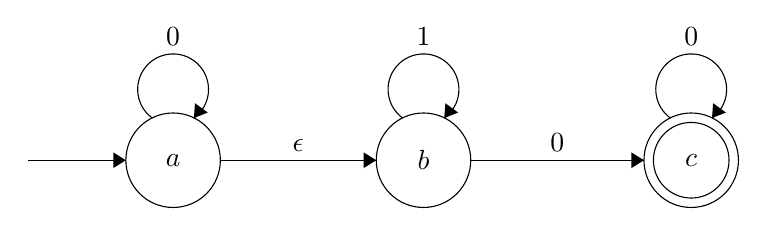
\begin{tikzpicture}[scale=0.2]
\tikzstyle{every node}+=[inner sep=0pt]
\draw [black] (10.6,-10.2) circle (3);
\draw (10.6,-10.2) node {$a$};
\draw [black] (26.5,-10.2) circle (3);
\draw (26.5,-10.2) node {$b$};
\draw [black] (43.5,-10.2) circle (3);
\draw (43.5,-10.2) node {$c$};
\draw [black] (43.5,-10.2) circle (2.4);
\draw [black] (9.277,-7.52) arc (234:-54:2.25);
\draw (10.6,-2.95) node [above] {$0$};
\fill [black] (11.92,-7.52) -- (12.8,-7.17) -- (11.99,-6.58);
\draw [black] (13.6,-10.2) -- (23.5,-10.2);
\fill [black] (23.5,-10.2) -- (22.7,-9.7) -- (22.7,-10.7);
\draw (18.55,-9.7) node [above] {$\epsilon$};
\draw [black] (25.177,-7.52) arc (234:-54:2.25);
\draw (26.5,-2.95) node [above] {$1$};
\fill [black] (27.82,-7.52) -- (28.7,-7.17) -- (27.89,-6.58);
\draw [black] (29.5,-10.2) -- (40.5,-10.2);
\fill [black] (40.5,-10.2) -- (39.7,-9.7) -- (39.7,-10.7);
\draw (35,-9.7) node [above] {$0$};
\draw [black] (42.177,-7.52) arc (234:-54:2.25);
\draw (43.5,-2.95) node [above] {$0$};
\fill [black] (44.82,-7.52) -- (45.7,-7.17) -- (44.89,-6.58);
\draw [black] (1.4,-10.2) -- (7.6,-10.2);
\fill [black] (7.6,-10.2) -- (6.8,-9.7) -- (6.8,-10.7);
\end{tikzpicture}
\end{center}
\end{homeworkProblem}

\begin{homeworkProblem}

\textbf{1.12}
\begin{center}
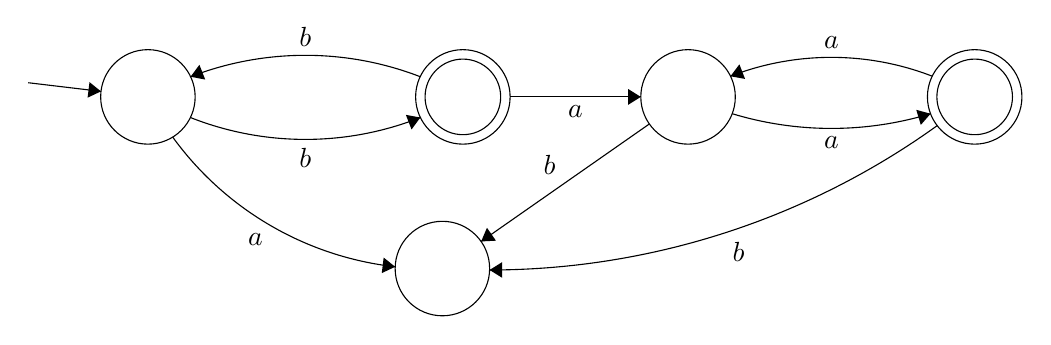
\begin{tikzpicture}[scale=0.2]
\tikzstyle{every node}+=[inner sep=0pt]
\draw [black] (8.3,-6.2) circle (3);
\draw [black] (28.3,-6.2) circle (3);
\draw [black] (28.3,-6.2) circle (2.4);
\draw [black] (27,-17.1) circle (3);
\draw [black] (42.6,-6.2) circle (3);
\draw [black] (60.8,-6.2) circle (3);
\draw [black] (60.8,-6.2) circle (2.4);
\draw [black] (0.7,-5.3) -- (5.32,-5.85);
\fill [black] (5.32,-5.85) -- (4.59,-5.26) -- (4.47,-6.25);
\draw [black] (24.005,-16.987) arc (-96.40192:-144.07284:20.237);
\fill [black] (24,-16.99) -- (23.27,-16.4) -- (23.15,-17.39);
\draw (15.13,-14.86) node [below] {$a$};
\draw [black] (25.604,-7.509) arc (-68.43209:-111.56791:19.869);
\fill [black] (25.6,-7.51) -- (24.68,-7.34) -- (25.04,-8.27);
\draw (18.3,-9.4) node [below] {$b$};
\draw [black] (11.009,-4.917) arc (111.10518:68.89482:20.249);
\fill [black] (11.01,-4.92) -- (11.94,-5.1) -- (11.57,-4.16);
\draw (18.3,-3.06) node [above] {$b$};
\draw [black] (31.3,-6.2) -- (39.6,-6.2);
\fill [black] (39.6,-6.2) -- (38.8,-5.7) -- (38.8,-6.7);
\draw (35.45,-6.7) node [below] {$a$};
\draw [black] (40.14,-7.92) -- (29.46,-15.38);
\fill [black] (29.46,-15.38) -- (30.4,-15.33) -- (29.83,-14.51);
\draw (33.8,-11.15) node [above] {$b$};
\draw [black] (57.999,-7.267) arc (-73.11305:-106.88695:21.683);
\fill [black] (58,-7.27) -- (57.09,-7.02) -- (57.38,-7.98);
\draw (51.7,-8.7) node [below] {$a$};
\draw [black] (45.293,-4.886) arc (111.16929:68.83071:17.742);
\fill [black] (45.29,-4.89) -- (46.22,-5.06) -- (45.86,-4.13);
\draw (51.7,-3.19) node [above] {$a$};
\draw [black] (58.42,-8.025) arc (-54.28428:-89.96823:48.733);
\fill [black] (30,-17.19) -- (30.8,-17.69) -- (30.8,-16.69);
\draw (45.8,-15.38) node [below] {$b$};
\end{tikzpicture}
\end{center}

\end{homeworkProblem}

\begin{homeworkProblem}
\textbf{1.21}
\begin{center}
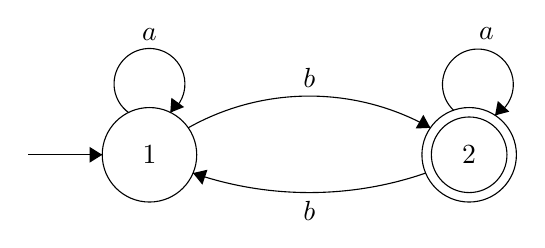
\begin{tikzpicture}[scale=0.2]
\tikzstyle{every node}+=[inner sep=0pt]
\draw [black] (8.5,-9.7) circle (3);
\draw (8.5,-9.7) node {$1$};
\draw [black] (28.8,-9.7) circle (3);
\draw (28.8,-9.7) node {$2$};
\draw [black] (28.8,-9.7) circle (2.4);
\draw [black] (0.8,-9.7) -- (5.5,-9.7);
\fill [black] (5.5,-9.7) -- (4.7,-9.2) -- (4.7,-10.2);
\draw [black] (7.177,-7.02) arc (234:-54:2.25);
\draw (8.5,-2.45) node [above] {$a$};
\fill [black] (9.82,-7.02) -- (10.7,-6.67) -- (9.89,-6.08);
\draw [black] (10.958,-7.988) arc (119.38377:60.61623:15.677);
\fill [black] (26.34,-7.99) -- (25.89,-7.16) -- (25.4,-8.03);
\draw (18.65,-5.47) node [above] {$b$};
\draw [black] (26.037,-10.862) arc (-70.97721:-109.02279:22.663);
\fill [black] (11.26,-10.86) -- (11.86,-11.6) -- (12.18,-10.65);
\draw (18.65,-12.6) node [below] {$b$};
\draw [black] (27.818,-6.878) arc (226.92001:-61.07999:2.25);
\draw (29.89,-2.42) node [above] {$a$};
\fill [black] (30.44,-7.2) -- (31.35,-6.96) -- (30.62,-6.28);
\end{tikzpicture}
\end{center}

\begin{center}
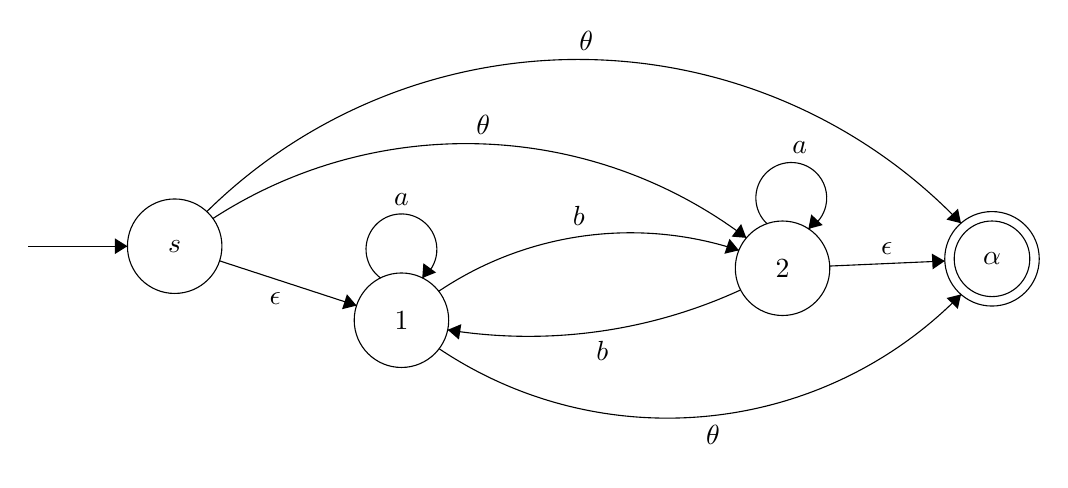
\begin{tikzpicture}[scale=0.2]
\tikzstyle{every node}+=[inner sep=0pt]
\draw [black] (28.7,-19.7) circle (3);
\draw (28.7,-19.7) node {$1$};
\draw [black] (52.9,-16.4) circle (3);
\draw (52.9,-16.4) node {$2$};
\draw [black] (14.3,-15) circle (3);
\draw (14.3,-15) node {$s$};
\draw [black] (66.2,-15.8) circle (3);
\draw (66.2,-15.8) node {$\alpha$};
\draw [black] (66.2,-15.8) circle (2.4);
\draw [black] (27.377,-17.02) arc (234:-54:2.25);
\draw (28.7,-12.45) node [above] {$a$};
\fill [black] (30.02,-17.02) -- (30.9,-16.67) -- (30.09,-16.08);
\draw [black] (31.067,-17.86) arc (123.92448:71.60585:21.817);
\fill [black] (50.13,-15.26) -- (49.53,-14.53) -- (49.21,-15.48);
\draw (39.97,-13.75) node [above] {$b$};
\draw [black] (50.236,-17.777) arc (-65.32404:-99.14563:32.269);
\fill [black] (31.64,-20.31) -- (32.35,-20.93) -- (32.5,-19.95);
\draw (41.45,-21.02) node [below] {$b$};
\draw [black] (51.918,-13.578) arc (226.92001:-61.07999:2.25);
\draw (53.99,-9.12) node [above] {$a$};
\fill [black] (54.54,-13.9) -- (55.45,-13.66) -- (54.72,-12.98);
\draw [black] (17.15,-15.93) -- (25.85,-18.77);
\fill [black] (25.85,-18.77) -- (25.24,-18.05) -- (24.93,-19);
\draw (20.69,-17.89) node [below] {$\epsilon$};
\draw [black] (5,-15) -- (11.3,-15);
\fill [black] (11.3,-15) -- (10.5,-14.5) -- (10.5,-15.5);
\draw [black] (55.9,-16.26) -- (63.2,-15.94);
\fill [black] (63.2,-15.94) -- (62.38,-15.47) -- (62.43,-16.47);
\draw (59.51,-15.56) node [above] {$\epsilon$};
\draw [black] (64.233,-18.063) arc (-44.30007:-123.82509:26.048);
\fill [black] (64.23,-18.06) -- (63.32,-18.29) -- (64.03,-18.98);
\draw (48.48,-26.36) node [below] {$\theta$};
\draw [black] (16.341,-12.802) arc (134.56517:43.66863:33.604);
\fill [black] (64.23,-13.54) -- (64.04,-12.62) -- (63.31,-13.31);
\draw (40.44,-2.63) node [above] {$\theta$};
\draw [black] (16.729,-13.241) arc (122.99256:52.85309:29.499);
\fill [black] (50.6,-14.47) -- (50.27,-13.59) -- (49.67,-14.39);
\draw (33.89,-7.97) node [above] {$\theta$};
\end{tikzpicture}
\end{center}

\begin{center}
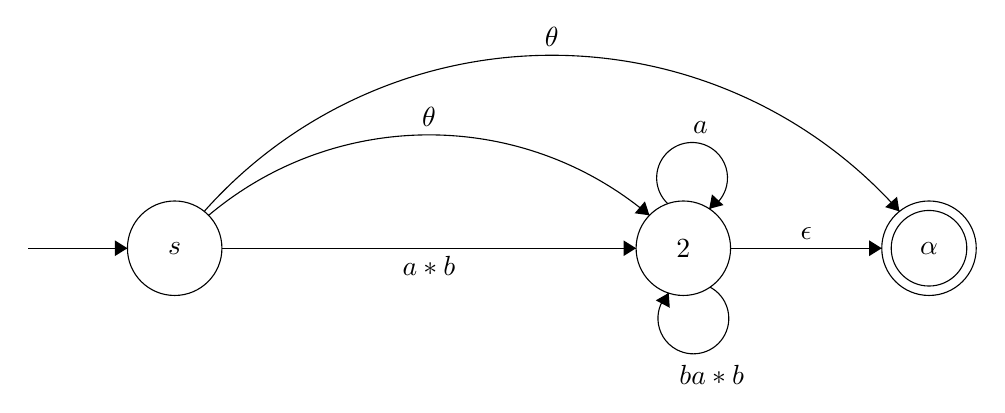
\begin{tikzpicture}[scale=0.2]
\tikzstyle{every node}+=[inner sep=0pt]
\draw [black] (46.6,-15) circle (3);
\draw (46.6,-15) node {$2$};
\draw [black] (14.3,-15) circle (3);
\draw (14.3,-15) node {$s$};
\draw [black] (62.2,-15) circle (3);
\draw (62.2,-15) node {$\alpha$};
\draw [black] (62.2,-15) circle (2.4);
\draw [black] (45.618,-12.178) arc (226.92001:-61.07999:2.25);
\draw (47.69,-7.72) node [above] {$a$};
\fill [black] (48.24,-12.5) -- (49.15,-12.26) -- (48.42,-11.58);
\draw [black] (5,-15) -- (11.3,-15);
\fill [black] (11.3,-15) -- (10.5,-14.5) -- (10.5,-15.5);
\draw [black] (49.6,-15) -- (59.2,-15);
\fill [black] (59.2,-15) -- (58.4,-14.5) -- (58.4,-15.5);
\draw (54.4,-14.5) node [above] {$\epsilon$};
\draw [black] (16.176,-12.66) arc (138.37374:41.62626:29.531);
\fill [black] (60.32,-12.66) -- (60.17,-11.73) -- (59.42,-12.39);
\draw (38.25,-2.25) node [above] {$\theta$};
\draw [black] (16.453,-12.914) arc (130.13427:49.86573:21.715);
\fill [black] (44.45,-12.91) -- (44.16,-12.02) -- (43.51,-12.78);
\draw (30.45,-7.3) node [above] {$\theta$};
\draw [black] (17.3,-15) -- (43.6,-15);
\fill [black] (43.6,-15) -- (42.8,-14.5) -- (42.8,-15.5);
\draw (30.45,-15.5) node [below] {$a*b$};
\draw [black] (48.288,-17.466) arc (62.1301:-225.8699:2.25);
\draw (48.4,-22.41) node [below] {$ba*b$};
\fill [black] (45.67,-17.84) -- (44.85,-18.31) -- (45.74,-18.78);
\end{tikzpicture}
\end{center}

\begin{center}
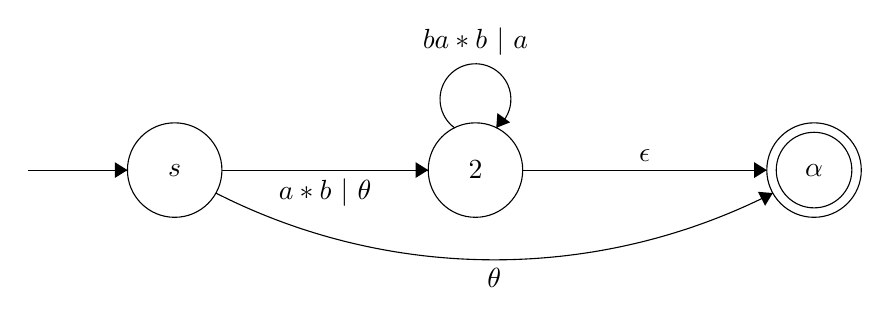
\begin{tikzpicture}[scale=0.2]
\tikzstyle{every node}+=[inner sep=0pt]
\draw [black] (31.6,-9.7) circle (3);
\draw (31.6,-9.7) node {$2$};
\draw [black] (12.5,-9.7) circle (3);
\draw (12.5,-9.7) node {$s$};
\draw [black] (53.1,-9.7) circle (3);
\draw (53.1,-9.7) node {$\alpha$};
\draw [black] (53.1,-9.7) circle (2.4);
\draw [black] (3.2,-9.7) -- (9.5,-9.7);
\fill [black] (9.5,-9.7) -- (8.7,-9.2) -- (8.7,-10.2);
\draw [black] (34.6,-9.7) -- (50.1,-9.7);
\fill [black] (50.1,-9.7) -- (49.3,-9.2) -- (49.3,-10.2);
\draw (42.35,-9.2) node [above] {$\epsilon$};
\draw [black] (50.481,-11.162) arc (-63.03923:-116.96077:38.998);
\fill [black] (50.48,-11.16) -- (49.54,-11.08) -- (49.99,-11.97);
\draw (32.8,-15.9) node [below] {$\theta$};
\draw [black] (15.5,-9.7) -- (28.6,-9.7);
\fill [black] (28.6,-9.7) -- (27.8,-9.2) -- (27.8,-10.2);
\draw (22.05,-10.2) node [below] {$a*b\mbox{ }|\mbox{ }\theta$};
\draw [black] (30.277,-7.02) arc (234:-54:2.25);
\draw (31.6,-2.45) node [above] {$ba*b\mbox{ }|\mbox{ }a$};
\fill [black] (32.92,-7.02) -- (33.8,-6.67) -- (32.99,-6.08);
\end{tikzpicture}
\end{center}

\begin{center}
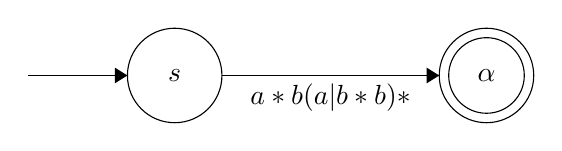
\begin{tikzpicture}[scale=0.2]
\tikzstyle{every node}+=[inner sep=0pt]
\draw [black] (12.5,-9.7) circle (3);
\draw (12.5,-9.7) node {$s$};
\draw [black] (32.3,-9.7) circle (3);
\draw (32.3,-9.7) node {$\alpha$};
\draw [black] (32.3,-9.7) circle (2.4);
\draw [black] (3.2,-9.7) -- (9.5,-9.7);
\fill [black] (9.5,-9.7) -- (8.7,-9.2) -- (8.7,-10.2);
\draw [black] (15.5,-9.7) -- (29.3,-9.7);
\fill [black] (29.3,-9.7) -- (28.5,-9.2) -- (28.5,-10.2);
\draw (22.4,-10.2) node [below] {$a*b(a|b*b)*$};
\end{tikzpicture}
\end{center}
\end{homeworkProblem}


\begin{homeworkProblem}
\textbf{1.28b} \\

Convert the following regular expression to NFA using the procedure given in Theorem 1.54. 
In all parts, $\sum = \{a,b\}$. \\

$a^+ | (ab)^+$

\begin{center}
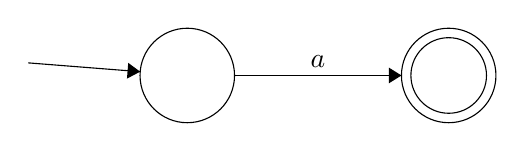
\begin{tikzpicture}[scale=0.2]
\tikzstyle{every node}+=[inner sep=0pt]
\draw [black] (13.3,-6) circle (3);
\draw [black] (29.9,-6) circle (3);
\draw [black] (29.9,-6) circle (2.4);
\draw [black] (3.2,-5.2) -- (10.31,-5.76);
\fill [black] (10.31,-5.76) -- (9.55,-5.2) -- (9.47,-6.2);
\draw [black] (16.3,-6) -- (26.9,-6);
\fill [black] (26.9,-6) -- (26.1,-5.5) -- (26.1,-6.5);
\draw (21.6,-5.5) node [above] {$a$};
\end{tikzpicture}
\end{center}

\begin{center}
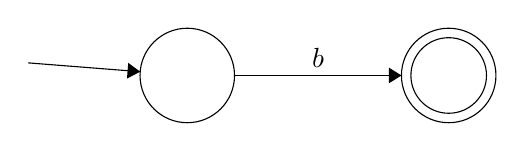
\begin{tikzpicture}[scale=0.2]
\tikzstyle{every node}+=[inner sep=0pt]
\draw [black] (13.3,-6) circle (3);
\draw [black] (29.9,-6) circle (3);
\draw [black] (29.9,-6) circle (2.4);
\draw [black] (3.2,-5.2) -- (10.31,-5.76);
\fill [black] (10.31,-5.76) -- (9.55,-5.2) -- (9.47,-6.2);
\draw [black] (16.3,-6) -- (26.9,-6);
\fill [black] (26.9,-6) -- (26.1,-5.5) -- (26.1,-6.5);
\draw (21.6,-5.5) node [above] {$b$};
\end{tikzpicture}
\end{center}

\begin{center}
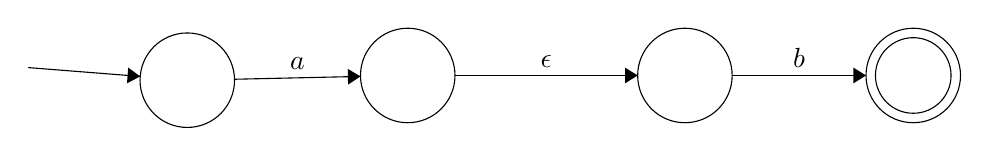
\begin{tikzpicture}[scale=0.2]
\tikzstyle{every node}+=[inner sep=0pt]
\draw [black] (13.3,-6) circle (3);
\draw [black] (27.3,-5.7) circle (3);
\draw [black] (44.9,-5.7) circle (3);
\draw [black] (59.4,-5.7) circle (3);
\draw [black] (59.4,-5.7) circle (2.4);
\draw [black] (3.2,-5.2) -- (10.31,-5.76);
\fill [black] (10.31,-5.76) -- (9.55,-5.2) -- (9.47,-6.2);
\draw [black] (16.3,-5.94) -- (24.3,-5.76);
\fill [black] (24.3,-5.76) -- (23.49,-5.28) -- (23.51,-6.28);
\draw (20.29,-5.33) node [above] {$a$};
\draw [black] (30.3,-5.7) -- (41.9,-5.7);
\fill [black] (41.9,-5.7) -- (41.1,-5.2) -- (41.1,-6.2);
\draw (36.1,-5.2) node [above] {$\epsilon$};
\draw [black] (47.9,-5.7) -- (56.4,-5.7);
\fill [black] (56.4,-5.7) -- (55.6,-5.2) -- (55.6,-6.2);
\draw (52.15,-5.2) node [above] {$b$};
\end{tikzpicture}
\end{center}

\begin{center}
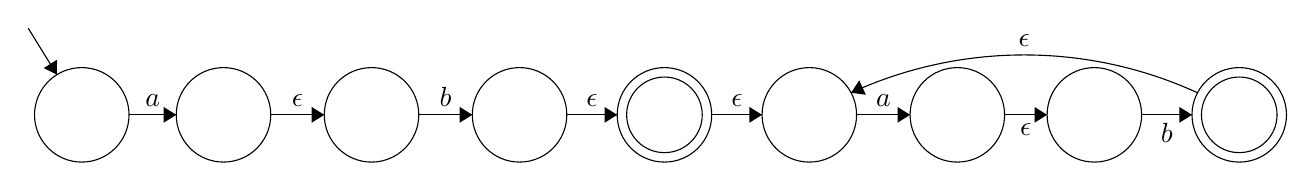
\begin{tikzpicture}[scale=0.2]
\tikzstyle{every node}+=[inner sep=0pt]
\draw [black] (3.4,-6.3) circle (3);
\draw [black] (12.4,-6.3) circle (3);
\draw [black] (21.8,-6.3) circle (3);
\draw [black] (31.2,-6.3) circle (3);
\draw [black] (40.4,-6.3) circle (3);
\draw [black] (40.4,-6.3) circle (2.4);
\draw [black] (67.7,-6.3) circle (3);
\draw [black] (76.9,-6.3) circle (3);
\draw [black] (76.9,-6.3) circle (2.4);
\draw [black] (49.6,-6.3) circle (3);
\draw [black] (59,-6.3) circle (3);
\draw [black] (0,-0.8) -- (1.82,-3.75);
\fill [black] (1.82,-3.75) -- (1.83,-2.8) -- (0.98,-3.33);
\draw [black] (6.4,-6.3) -- (9.4,-6.3);
\fill [black] (9.4,-6.3) -- (8.6,-5.8) -- (8.6,-6.8);
\draw (7.9,-5.8) node [above] {$a$};
\draw [black] (15.4,-6.3) -- (18.8,-6.3);
\fill [black] (18.8,-6.3) -- (18,-5.8) -- (18,-6.8);
\draw (17.1,-5.8) node [above] {$\epsilon$};
\draw [black] (24.8,-6.3) -- (28.2,-6.3);
\fill [black] (28.2,-6.3) -- (27.4,-5.8) -- (27.4,-6.8);
\draw (26.5,-5.8) node [above] {$b$};
\draw [black] (34.2,-6.3) -- (37.4,-6.3);
\fill [black] (37.4,-6.3) -- (36.6,-5.8) -- (36.6,-6.8);
\draw (35.8,-5.8) node [above] {$\epsilon$};
\draw [black] (70.7,-6.3) -- (73.9,-6.3);
\fill [black] (73.9,-6.3) -- (73.1,-5.8) -- (73.1,-6.8);
\draw (72.3,-6.8) node [below] {$b$};
\draw [black] (43.4,-6.3) -- (46.6,-6.3);
\fill [black] (46.6,-6.3) -- (45.8,-5.8) -- (45.8,-6.8);
\draw (45,-5.8) node [above] {$\epsilon$};
\draw [black] (52.6,-6.3) -- (56,-6.3);
\fill [black] (56,-6.3) -- (55.2,-5.8) -- (55.2,-6.8);
\draw (54.3,-5.8) node [above] {$a$};
\draw [black] (62,-6.3) -- (64.7,-6.3);
\fill [black] (64.7,-6.3) -- (63.9,-5.8) -- (63.9,-6.8);
\draw (63.35,-6.8) node [below] {$\epsilon$};
\draw [black] (52.25,-4.897) arc (114.63693:65.36307:26.387);
\fill [black] (52.25,-4.9) -- (53.19,-5.02) -- (52.77,-4.11);
\draw (63.25,-2) node [above] {$\epsilon$};
\end{tikzpicture}
\end{center}


\begin{center}
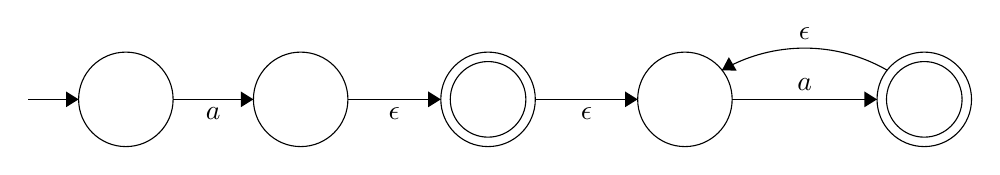
\begin{tikzpicture}[scale=0.2]
\tikzstyle{every node}+=[inner sep=0pt]
\draw [black] (7.7,-6.1) circle (3);
\draw [black] (18.8,-6.1) circle (3);
\draw [black] (30.7,-6.1) circle (3);
\draw [black] (30.7,-6.1) circle (2.4);
\draw [black] (43.2,-6.1) circle (3);
\draw [black] (58.4,-6.1) circle (3);
\draw [black] (58.4,-6.1) circle (2.4);
\draw [black] (10.7,-6.1) -- (15.8,-6.1);
\fill [black] (15.8,-6.1) -- (15,-5.6) -- (15,-6.6);
\draw (13.25,-6.6) node [below] {$a$};
\draw [black] (21.8,-6.1) -- (27.7,-6.1);
\fill [black] (27.7,-6.1) -- (26.9,-5.6) -- (26.9,-6.6);
\draw (24.75,-6.6) node [below] {$\epsilon$};
\draw [black] (33.7,-6.1) -- (40.2,-6.1);
\fill [black] (40.2,-6.1) -- (39.4,-5.6) -- (39.4,-6.6);
\draw (36.95,-6.6) node [below] {$\epsilon$};
\draw [black] (46.2,-6.1) -- (55.4,-6.1);
\fill [black] (55.4,-6.1) -- (54.6,-5.6) -- (54.6,-6.6);
\draw (50.8,-5.6) node [above] {$a$};
\draw [black] (45.55,-4.252) arc (120.00385:59.99615:10.499);
\fill [black] (45.55,-4.25) -- (46.49,-4.28) -- (45.99,-3.42);
\draw (50.8,-2.34) node [above] {$\epsilon$};
\draw [black] (1.5,-6.1) -- (4.7,-6.1);
\fill [black] (4.7,-6.1) -- (3.9,-5.6) -- (3.9,-6.6);
\end{tikzpicture}
\end{center}

\begin{center}
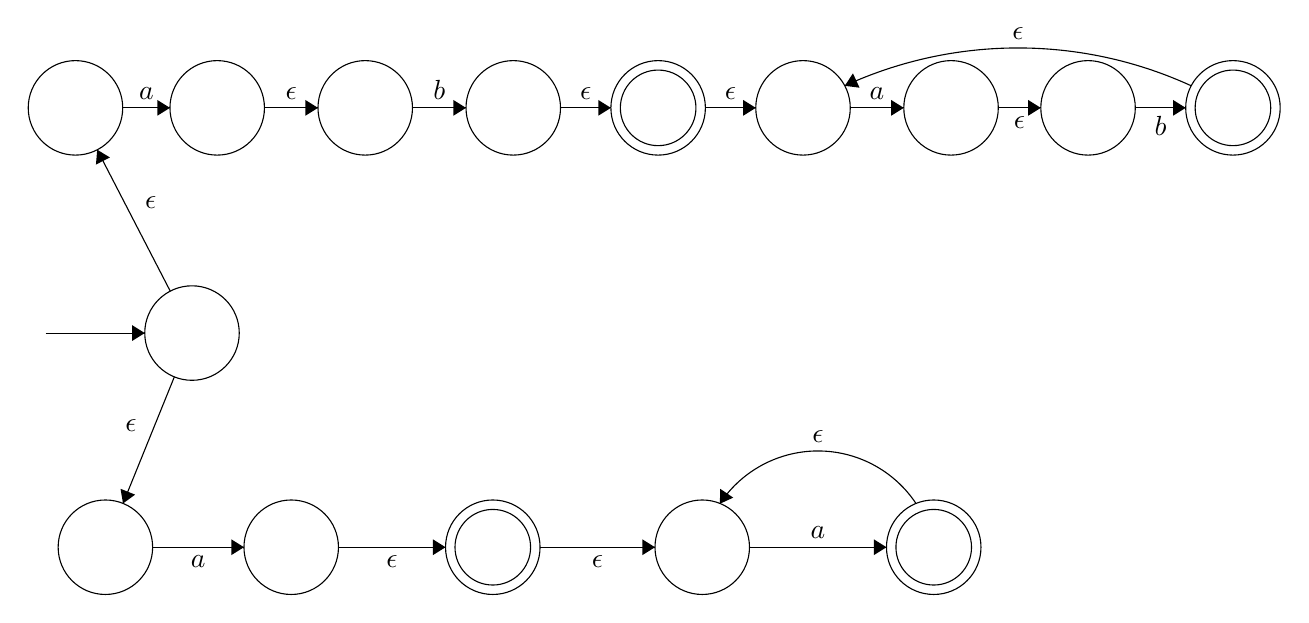
\begin{tikzpicture}[scale=0.2]
\tikzstyle{every node}+=[inner sep=0pt]
\draw [black] (3.4,-6.3) circle (3);
\draw [black] (12.4,-6.3) circle (3);
\draw [black] (21.8,-6.3) circle (3);
\draw [black] (31.2,-6.3) circle (3);
\draw [black] (40.4,-6.3) circle (3);
\draw [black] (40.4,-6.3) circle (2.4);
\draw [black] (67.7,-6.3) circle (3);
\draw [black] (76.9,-6.3) circle (3);
\draw [black] (76.9,-6.3) circle (2.4);
\draw [black] (49.6,-6.3) circle (3);
\draw [black] (59,-6.3) circle (3);
\draw [black] (10.8,-20.6) circle (3);
\draw [black] (5.3,-34.2) circle (3);
\draw [black] (17.1,-34.2) circle (3);
\draw [black] (29.9,-34.2) circle (3);
\draw [black] (29.9,-34.2) circle (2.4);
\draw [black] (43.2,-34.2) circle (3);
\draw [black] (57.9,-34.2) circle (3);
\draw [black] (57.9,-34.2) circle (2.4);
\draw [black] (6.4,-6.3) -- (9.4,-6.3);
\fill [black] (9.4,-6.3) -- (8.6,-5.8) -- (8.6,-6.8);
\draw (7.9,-5.8) node [above] {$a$};
\draw [black] (15.4,-6.3) -- (18.8,-6.3);
\fill [black] (18.8,-6.3) -- (18,-5.8) -- (18,-6.8);
\draw (17.1,-5.8) node [above] {$\epsilon$};
\draw [black] (24.8,-6.3) -- (28.2,-6.3);
\fill [black] (28.2,-6.3) -- (27.4,-5.8) -- (27.4,-6.8);
\draw (26.5,-5.8) node [above] {$b$};
\draw [black] (34.2,-6.3) -- (37.4,-6.3);
\fill [black] (37.4,-6.3) -- (36.6,-5.8) -- (36.6,-6.8);
\draw (35.8,-5.8) node [above] {$\epsilon$};
\draw [black] (70.7,-6.3) -- (73.9,-6.3);
\fill [black] (73.9,-6.3) -- (73.1,-5.8) -- (73.1,-6.8);
\draw (72.3,-6.8) node [below] {$b$};
\draw [black] (43.4,-6.3) -- (46.6,-6.3);
\fill [black] (46.6,-6.3) -- (45.8,-5.8) -- (45.8,-6.8);
\draw (45,-5.8) node [above] {$\epsilon$};
\draw [black] (52.6,-6.3) -- (56,-6.3);
\fill [black] (56,-6.3) -- (55.2,-5.8) -- (55.2,-6.8);
\draw (54.3,-5.8) node [above] {$a$};
\draw [black] (62,-6.3) -- (64.7,-6.3);
\fill [black] (64.7,-6.3) -- (63.9,-5.8) -- (63.9,-6.8);
\draw (63.35,-6.8) node [below] {$\epsilon$};
\draw [black] (52.25,-4.897) arc (114.63693:65.36307:26.387);
\fill [black] (52.25,-4.9) -- (53.19,-5.02) -- (52.77,-4.11);
\draw (63.25,-2) node [above] {$\epsilon$};
\draw [black] (1.5,-20.6) -- (7.8,-20.6);
\fill [black] (7.8,-20.6) -- (7,-20.1) -- (7,-21.1);
\draw [black] (9.42,-17.94) -- (4.78,-8.96);
\fill [black] (4.78,-8.96) -- (4.7,-9.9) -- (5.59,-9.45);
\draw (7.79,-12.31) node [right] {$\epsilon$};
\draw [black] (9.68,-23.38) -- (6.42,-31.42);
\fill [black] (6.42,-31.42) -- (7.19,-30.86) -- (6.26,-30.49);
\draw (7.31,-26.5) node [left] {$\epsilon$};
\draw [black] (8.3,-34.2) -- (14.1,-34.2);
\fill [black] (14.1,-34.2) -- (13.3,-33.7) -- (13.3,-34.7);
\draw (11.2,-34.7) node [below] {$a$};
\draw [black] (20.1,-34.2) -- (26.9,-34.2);
\fill [black] (26.9,-34.2) -- (26.1,-33.7) -- (26.1,-34.7);
\draw (23.5,-34.7) node [below] {$\epsilon$};
\draw [black] (32.9,-34.2) -- (40.2,-34.2);
\fill [black] (40.2,-34.2) -- (39.4,-33.7) -- (39.4,-34.7);
\draw (36.55,-34.7) node [below] {$\epsilon$};
\draw [black] (46.2,-34.2) -- (54.9,-34.2);
\fill [black] (54.9,-34.2) -- (54.1,-33.7) -- (54.1,-34.7);
\draw (50.55,-33.7) node [above] {$a$};
\draw [black] (44.316,-31.437) arc (146.51092:33.48908:7.475);
\fill [black] (44.32,-31.44) -- (45.17,-31.05) -- (44.34,-30.49);
\draw (50.55,-27.59) node [above] {$\epsilon$};
\end{tikzpicture}
\end{center}


\end{homeworkProblem}



\begin{homeworkProblem}
\textbf{1.29b} \\
Use the pumping lemma to show that the following languages are not regular. \\ 
$A_2 = \{www| w \in \{a,b\}^*\}$\\

Assume that $A_2 = \{www| w \in \{a,b\}^*\}$\\ is regular. Let p be the pumping 
length given by the pumping lemma. Choose $s$ to be the string $a^pba^pba^pb$. 
Because s is a member of $A_2$ and $s$ is longer than p, the pumping lemma guarantees 
that $s$ can be split into three pieces, $s=xyz$, where $|xy| \leq p$, hence $y$ can 
only be contained in first $a^p$. Since $y \geq 1$, let $y = a^i$, $i > 0$. 
However, $xy^2z = a^{p+k}ba^pba^pb$, where $p+k > P$, is not in $A_2$. That is $s$ 
cannot be pumped. This is a contradiction. Thus, $A_2$ is not regular.

\end{homeworkProblem}
\begin{homeworkProblem}
\textbf{1.31} \\
For any string $ w = w_qw_2\cdot w_n$, the reverse of $w$, written $w^R$, is the string $w$ in reverse order, 
$w_n\cdots w_2 w_1$.  For any language $A$, let $A^R = \{w^R | w \in A\}$.
Show that if $A$ is regular, so is $A^R$.\\

By theorem if $A$ is regular, then there is a DFA $M = (Q,\sum, \delta, q_0, F)$ such that $M$ recognizes $A$. 
We will show that it is possible to construct
an NFA $N = (Q',\sum ', \delta ', q_0 ', F ')$ that will recognize $A^R$.

Informally:
\begin{enumerate}[1., leftmargin = 0.5cm, nosep]
\item Reverse all the connections in the automaton.
\item Add a new state $q_f$
\item Draw $\epsilon$ connection from state $q_f$ to every final state.
\item Make all the final states normal states.
\item Make start state final state.
\item Make $q_f$ the start state. \\
\end{enumerate}
Formally
\begin{itemize}
\item $Q' = Q \cup \{q_0'\}$, where $q_0$ is the new start state
\item $F' = \{q_0\}$, is the new final state. We accept only in the start state of the original DFA.
\item Define transition functions $\delta'$.
\begin{equation}
  \delta(q,a) '=\begin{cases}
    F, & \text{if } q = q_0' \text{ and } a = \epsilon \\
    \delta^{-1}(q,a), & \text{if } q \neq q_0' \text{ and } a \neq \epsilon . \\
    \emptyset, & \text{otherwise}.
  \end{cases}
\end{equation}

\end{itemize}
By how we dfined $\delta ', q_0, q_1, \cdot, q_n$ is an accepting computation of $M$ on input $w_1w_2\cdot w_n$ if
and only if $q_0',q_n,\cdot ,q_1, q_0 $ is an accepting computation of $N$ on input $w_n \cdot w_2 w_1$ (since
$\delta(q_i,w_{i+1} = q_{i+i} iff q_i \in \delta' (q_{i+1},w_{i+1})$ for $0 \leq i < n$ and 
$q_n \in \delta'(q_0', \epsilon))$. Thus, $N$ recognizes $A^R$. Since for any regular language $A$ there exists an NFA that recognizes
$A^R$, we conclude that the class of regular languages is closed under reverse.
\end{homeworkProblem}

\begin{homeworkProblem}
\textbf{1.32}
\end{homeworkProblem}

Let $w^R$ denote the reverse of the string $w$. For any language A, let $A^R = \{w^R | w\in A\}$.
Then if $A$ is regular, so is $A^R$.
\\
Now, the construction of the automata for the language $B^R$ is simple. We get columns of size 3
as our alphabets at each stage, we will need to keep track of two things, wheter there is a carry or not. Depending on wheter there
was a carry or not, we just need to verify that the provided 3-column is consistent. \\

Figure 4 shows that NFA for $B^R$.

\begin{homeworkProblem}
\textbf{1.46c}\\
$L = \{w|w \in \{0,1\}^* \text{ is not a palindrome }\}$ \\

We can show that $L$ is not regular, by showing that it's compliment
$L' = \{w|w \in \{0,1\}^* \text{ is a palindrome }\}$ is not regular. \\
Choose $s = 0^p10^p = xyz,\text{ a palindrome in } L'$. Here $xy$ contains only 0's.
Let $y = 0^k, k>0$. Thus $xy^0z = 0^{p-k}10^p$ is not in the language. Thus, it's not regular.


\end{homeworkProblem}
%\begin{homeworkProblem}
%\end{homeworkProblem}
\end{document}
